  
\RequirePackage{fix-cm}
\documentclass[smallextended]{svjour3}       % onecolumn (second format)
\smartqed  % flush right qed marks, e.g. at end of proof
\usepackage{stmaryrd}
\usepackage{citesort}
\usepackage{bussproofs}
\usepackage{turnstile}
\usepackage{amssymb}
\usepackage{latexsym}
\setcounter{tocdepth}{3}
\usepackage{graphicx}
\usepackage{url}
\usepackage{amsmath}
\usepackage{listings}
\usepackage{subfig}
\usepackage{pgf}
\usepackage{tikz}
\usetikzlibrary{arrows,shapes,snakes,automata,backgrounds,petri}
\usepackage[latin1]{inputenc}
\usepackage{float}
\usepackage{amssymb}


\usepackage{ifthen}
\usepackage{amssymb}
\newboolean{showcomments}
\setboolean{showcomments}{true}
\ifthenelse{\boolean{showcomments}}
  {\newcommand{\mynote}[2]{
    \fbox{\bfseries\sffamily\scriptsize#1}
    {\small$\blacktriangleright$\textsf{\emph{#2}}$\blacktriangleleft$}
   }
  }
  {\newcommand{\mynote}[2]{}
  }
\newcommand\laurie[1]{\mynote{Laurie}{#1}}
\newcommand\richard[1]{\mynote{Richard}{#1}}

\newcommand{\MAY}[2]{\langle #1 \rangle #2}
\newcommand{\NEG}[1]{\mathsf{neg}(#1)}
\newcommand{\AND}{\land}

\lstnewenvironment{code}
    {\lstset{}%
      \csname lst@SetFirstLabel\endcsname}
    {\csname lst@SaveFirstLabel\endcsname}
    \lstset{
      basicstyle=\small\ttfamily,
      flexiblecolumns=false,
      basewidth={0.5em,0.45em},
      literate={+}{{$+$}}1 {/}{{$/$}}1 {*}{{$*$}}1 {=}{{$=$}}1
               {>}{{$>$}}1 {<}{{$<$}}1 {\\}{{$\lambda$}}1
               {\\\\}{{\char`\\\char`\\}}1
               {->}{{$\rightarrow$}}2 {>=}{{$\geq$}}2 {<-}{{$\leftarrow$}}2
               {<=}{{$\leq$}}2 {=>}{{$\Rightarrow$}}2 
               {\ .}{{$\bigcirc$}}2 {\ .\ }{{$\bigcirc$}}2
               {>>}{{>>}}2 {>>=}{{>>=}}2
               {|}{{$\mid$}}1               
    }

\newtheorem{mycase}{Case}
\newtheorem{subcase}{Case}
\numberwithin{subcase}{mycase}


% Dot
\def\fDot {\ast}
% Bang
\def\fBang {\ ! \ }
% Or
\def\fOr {\ | \ }

% Turnstiles with subscripts
\def\judgeX {\sststile{\mathrm{X}}{}}
\def\judgeY {\sststile{\mathrm{Y}}{}}
\def\judge {\sststile{\mathrm{}}{}}

\EnableBpAbbreviations


\begin{document}

\title {Eremic Logic\footnote{Version of \today.}} 
\subtitle {A Modal Logic of Elementary Propositions}
\author{Richard Prideaux Evans \and  Martin Berger}
\institute {Richard Prideaux Evans,
\martin{Richard, but in your address} Oxford, Bla. \email{richardprideauxevans@gmail.com}
 \and Martin Berger, University of Sussex. \email{M.F.Berger@sussex.ac.uk}.}
\date{Received: date / Accepted: date}
% The correct dates will be entered by the editor



\bibliographystyle{abbrv} % I don't know what the JPL uses as bibliographic style. Using 
                          % abbrv for now.
\maketitle

\keywords{Modal logic, Hennessy-Milner logic, negation, \martin{Add more as required by the  JPL.}} 

\begin{abstract}
Eremic Logic is a simple modal logic for capturing inferences between ``atomic'' sentences. 
It is the only Hennessy-Milner style logic satisfying the Hennessy-Milner theorem that has a linear-time decision procedure.
It has been put to use in an industrial application, as the representational core of a new logic programming language. The resulting code is shorter, less error-prone, and more efficient than the corresponding code in traditional predicate logic.
\end{abstract}

\section{Stylistic conventions}

It is very helpful for the reader if variables names give some
indication about what they range over, e.g. a set $S$ is ranged over
by $s, s', s_1, s_2, ...$ etc.  It is also very helpful to be very
consistent in this regard.  This section proposes some such
conventions. The section will be removed before submission.

\begin{itemize}

\item Formulae  are ranged over by $\phi, \psi$ etc.
\item Integers are ranged over by $i, j, m, n, ...$ etc.
\item States are ranged over by $s, s', t, ...$ etc.
\item Actions are ranged over by $a, a', b, ...$ etc.
\item Simulations and bisimulations are ranged over by $\RRR$ etc.
\item LTS are ranged over by $\CAL{L}, ...$ etc.
\item Models are ranged over by $\FRAK{M}, ...$ etc.

\end{itemize}
 % to be removed later.
\section{Introduction}\label{introduction}

Natural language is full of incompatible alternatives.
If Pierre is the current king of France, then nobody else can simultaneously fill that role.
A traffic light can be green, amber or red - but it cannot be more than one colour at a time.
Mutual exclusion is a natural and ubiquitous concept.
\FOL{} can represent mutually exclusive alternatives, of course.
To say that Pierre is the only king of France, we can write, following Russell:
\[
king(france, pierre) \land \forall x . (king(france, x) \rightarrow x = pierre).
\]
To say that a particular traffic light, $tl$, is red - and red is its only colour - we could write:
\[
colour(tl, red) \land \forall x . colour(tl, x) \rightarrow x = red.
\]
In this approach, incompatibility is a \emph{derived} concept, reduced to 
a combination of universal quantification and identity.  
\FOL{}, in other words, uses relatively complex machinery to express a
simple concept:
\begin{itemize}

\item Quantification's complexity comes from the
  rules governing the distinction between free
  and bound variables.
  
\item Identity's complexity comes from the infinite collection of axioms required to formalise the
  indiscernibility of identicals.

\end{itemize}

\NI The costs of quantification and identity, such as a larger proof
search space, have to be borne every time one expresses a sentence that excludes others - even
though incompatibility does not, prima facie, appear to have anything to do
with the free/bound variable distinction, or require the full power of 
the identity relation.

This paper introduces an alternative approach, where
exclusion is expressed directly, as a first-class concept.
 \Cathoristic{}\footnote{``Cathoristic'' comes from the Greek
  $\kappa \alpha \theta o \rho \acute{\i} \zeta \epsilon i \nu$: to impose narrow
  boundaries. We are grateful to Tim Whitmarsh for suggesting this
  word.} is the simplest logic we could find in which incompatible
statements can be expressed.  
It is a multi-modal logic, a variant of Hennessy-Milner logic,
that replaces negation with a new logical primitive
\[
   !A
\]
pronounced \emph{tantum}\footnote{``Tantum'' is Latin for ``only''.}
$A$. Here $A$ is a finite set of alternatives, and $!A$ says that the
alternatives in $A$ exhaust all possibilities.  For example:
\begin{eqnarray*}
\fBang \{green, amber, red\}
\end{eqnarray*}
states that nothing but $green$, $amber$ or $red$ is possible.  Our
logic uses modalities to state facts, for example $\MAY{amber}{}$
expresses that $amber$ is currently the case.  The power of the logic
comes from the conjunction of modalities and tantum. For example
\[
   \MAY{amber}{}\ \AND\ !\{green, amber, red\} 
\]
expresses that $amber$ is currently the case and $red$ as well as
$green$ are the only two possible alternatives to $amber$.  Any
statement that exceeds what tantum $A$ allows, like
\[
   \MAY{blue} \ \AND\ !\{green, amber, red\},
\]
is necessarily false.  When the only options are green, amber, or red,
then blue is not permissible.  Now to say that Pierre is the only king
of France, we write:
\[
\MAY{king}\MAY{france}(\MAY{pierre} \land \fBang \{pierre\}).
\]
Crucially, \cathoristic{}'s representation involves no
universal quantifier and no identity relation.  It is a purely
propositional formulation.  To say that the traffic
light is currently red, and red is its only colour, we write:
\[
\MAY{tl} \MAY{colour} (\MAY{red} \land !\{red\}).
\]
This is simpler, both in terms of representation length and
computational complexity, than the formulation in \fol{} given on the
previous page.
%% \[
%% colour(tl, red) \land \forall x . colour(tl, x) \rightarrow x = red
%% \]
Properties changing over time can be expressed by adding extra
modalities that can be understood as time-stamps.  To say that that
the traffic light was red at time $t_1$ and amber at time $t_2$, we
can write:
\[
   \MAY{tl} \MAY{colour} (\MAY{t_1} (\MAY{red} \land !\{red\}) \land \MAY{t_2} (\MAY{amber} \land !\{amber\}))
\]
Change over time can be expressed in first-order logic with bounded
quantification - but modalities are succinct and avoid introducing
bound variables.

Having claimed that incompatibility is a natural logical concept, not
easily expressed in first-order logic\footnote{We will precisify this
  claim in later sections; (1) first-order logic's representation of
  incompatibility is longer in terms of formula length than
  \cathoristic{}'s (see Section \ref{incompatiblepredicatesinfol});
  and (2) logic programs in \cathoristic{} can be optimised to run
  significantly faster than their equivalent in \fol{} (see Section
  \ref{optimizingpreconditions}).}, we will now argue the following:

\begin{itemize}

\item Incompatibility is conceptually prior to negation.

\item Negation arises as the weakest form of incompatibility.

\end{itemize}

\subsection{Material incompatibility and negation}

\NI Every English speaker knows that
\begin{quote}
``Jack is alive'' is incompatible with ``Jack is dead''
\end{quote}

\NI But \emph{why} are these sentences incompatible? The orthodox
position is that these sentences are incompatible because of the
following general law:
\begin{quote}
If someone is alive, then it is not the case that they are dead
\end{quote}
Recast in first-order logic:
\[
\forall x. ( alive(x) \IMPLIES \neg dead(x) ).
\]

\NI In other words, according to the orthodox position, the
incompatibility between the two particular sentences depends on a
general law involving universal quantification, implication and
negation.

Brandom \cite{brandom2} follows Sellars in proposing an alternative explanation: ``Jack
is alive'' is incompatible with ``Jack is dead'' because ``is alive''
and ``is dead'' are \emph{materially incompatible} predicates.  They
claim we can understand incompatible predicates even if we do
not understand universal quantification or negation.  
Material incompatibility is conceptually prior to logical negation.

Imagine, to make this vivid, a primitive people speaking a primordial
language of atomic sentences\footnote{In this paper, we define a sentence as \emph{atomic} if it does
  not contain another sentence as a syntactic constituent.}. These people can express sentences
that \emph{are} incompatible.  But they cannot express \emph{that}
they are incompatible.  They recognise when atomic sentences are
incompatible, and see that one sentence entails another - but their
behaviour outreaches their ability to articulate it.

Over time, these people \emph{may} advance to a more sophisticated
language where incompatibilities are made explicit, using a negation
operator - but this is a later (and optional) development:
\begin{quote}
[If negation is added to the language], it lets one say that two
claims are materially incompatible:``If a monochromatic patch is red,
then it is not blue.'' That is, negation lets one make explicit in the
form of claims - something that can be said and (so) thought - a
relation that otherwise remained implicit in what one practically did,
namely treat two claims as materially
incompatible\footnote{\cite{brandom} pp.47-48}.
\end{quote}

\NI But before making this optional
explicating step, our primitive people understand incompatibility
without understanding negation.  If this picture of our primordial
language is coherent, then material incompatibility is conceptually
independent of logical negation.

Now imagine a modification of our primitive linguistic practice in
which no sentences are ever treated as incompatible.  If one person
says ``Jack is alive'' and another says ``Jack is dead'', nobody
counts these claims as \emph{conflicting}.  The native speakers never
disagree, back down, retract their claims, or justify them. They just
say things.  Without an understanding of incompatibility, and the
variety of behaviour that it engenders, we submit (following Brandom)
that there is insufficient richness in the linguistic practice for
their sounds to count as assertions.  Without material
incompatibility, their sounds are just \emph{barks}.
\begin{quote}

  Suppose the reporter's differential responsive dispositions to call
  things red are matched by those of a parrot trained to utter the
  same noises under the same stimulation. What practical capacities of
  the human distinguish the reporter from the parrot? What, besides
  the exercise of regular differential responsive dispositions, must
  one be able to \emph{do}, in order to count as having or grasping
  \emph{concepts}? ... To grasp or understand a concept is, according
  to Sellars, to have practical mastery over the inferences it is
  involved in... The parrot does not treat ``That's red'' as
  incompatible with ``That's green''\footnote{\cite{brandom2}
    pp.88-89, our emphasis.}.
\end{quote}

\NI If this claim is also accepted, then material incompatibility is
not just conceptually \emph{independent} of logical negation, but
conceptually \emph{prior}.  

\subsection{Negation as the minimal incompatible}

In \cite{brandom2} and \cite{brandom}, Brandom describes 
logical negation as a limiting form of material incompatibility:
\begin{quote}
Incompatible sentences are Aristotelian \emph{contraries}. A sentence
and its negation are \emph{contradictories}. What is the relation
between these? Well, the contradictory is a contrary: any sentence is
incompatible with its negation. What distinguishes the contradictory
of a sentence from all the rest of its contraries? The contradictory
is the \emph{minimal} contrary: the one that is entailed by all the
rest. Thus every contrary of ``Plane figure $f$ is a circle'' - for
instance ``$f$ is a triangle'', ``$f$ is an octagon'', and so on -
entails ``$f$ is \emph{not} a circle''.
\end{quote}

\NI If someone asserts that it is not the case that Pierre is the (only) King of France,
we have said very little.  There are so many different ways in which
it could be true:
\begin{itemize}
\item
The King of France might be Jacques
\item
The King of France might be Louis
\item
...
\item
There may be no King of France at all
\item
There may be no country denoted by the word ``France''
\end{itemize}
Each of these concrete propositions is incompatible with Pierre being the King of France.
To say ``It is not the case that the King of France is Pierre'' is just to claim that one of these indefinitely many concrete possibilities is true.
Negation is just the logically weakest form of incompatibility.

In the rest of this paper, we assume - without further argument - that material incompatibility is conceptually prior to logical negation.
We develop a simple
 modal logic to articulate Brandom's intuition: a language, without negation, in which we can nevertheless make incompatible claims.

\subsection{Inferences between atomic sentences}
\label{intrasentential}
So far, we have justified the claim that incompatibility is a
fundamental logical concept by arguing that incompatibility is
conceptually prior to negation.  Now incompatibility is an inferential
relation between \emph{atomic sentences}.  In this subsection, we
shall describe \emph{other} inferential relations between atomic
sentences - inferential relations that \fol{} cannot articulate (or
can only do so awkwardly), but that \cathoristic{} handles naturally.

The \emph{atomic sentences} of a natural language can be
characterised as the sentences which do not contain any other
sentences as constituent parts\footnote{Compare Russell \cite{russell}
  p.117: ``A sentence is of atomic form when it contains no logical
  words and no subordinate sentence''. We use a broader notion of
  atomicity by focusing solely on whether or not it contains a
  subordinate sentence, allowing logical words such as ``and'' \emph{as long
  as they are conjoining noun-phrases} and not sentences.}.  According
to this criterion, the following are atomic:

\begin{itemize}

\item Jack is alive
\item Jack loves Jill
\end{itemize}

\NI The following is not atomic:

\begin{quote}
  Jack is alive and Jill is dead
\end{quote}

\NI because it contains the complete sentence ``Jack is alive'' as a
syntactic constituent.  Note that, according to this criterion, the
following \emph{is} atomic, despite using ``and'':

\begin{quote}
  Jack loves Jill and Joan
\end{quote}

\NI Here, ``Jack loves Jill'' is not a syntactic constituent\footnote{To see that ``Jack loves Jill'' is not a constituent of ``Jack loves Jill and Joan'', observe that ``and'' conjoins constituents of the \emph{same syntactic type}. But ``Jack loves Jill'' is a sentence, while ``Joan'' is a noun. Hence the correct parsing is ``Jack (loves (Jill and Joan))'', rather than ``(Jack loves Jill) and Joan''.}.

There are many types of inferential relations between atomic
sentences of a natural language.  For example:

\begin{itemize}

\item ``Jack is alive'' is incompatible with ``Jack is dead''
\item ``Jack loves Jill'' implies ``Jack loves''
\item ``Jack walks slowly'' implies ``Jack walks''
\item ``Jack loves Jill and Joan'' implies ``Jack loves Jill''
\item ``Jack is wet and cold'' implies ``Jack is cold''

\end{itemize}

\NI The first of these examples involves an incompatibility relation,
while the others involve entailment relations.  A key question this
paper seeks to answer is: what is the simplest logic that can capture
these inferential relations between atomic sentences?

\subsection{Wittgenstein's vision of a logic of elementary propositions}

\NI In the \emph{Tractatus} \cite{wittgenstein-tractatus}, Wittgenstein
claims that the world is a set of atomic sentences in an idealised
logical language.  Each atomic sentence was supposed to be
\emph{logically independent} of every other, so that they could be
combined together in every possible permutation, without worrying
about their mutual compatibility.
But already there were doubts and problem cases.  He was aware that
certain  statements seemed atomic, but did not seem logically
independent:

\begin{quote}
  For two colours, e.g., to be at one place in the visual field is
  impossible, and indeed logically impossible, for it is excluded by
  the logical structure of colour. (6.3751)
\end{quote}

\NI At the time of writing the \emph{Tractatus}, he hoped that further
analysis would reveal that these statements were not really atomic.

Later, in the \emph{Philosophical Remarks} \cite{wittgenstein-remarks}, he
renounced the thesis of the logical independence of atomic
propositions.  In \S 76, talking about incompatible colour predicates,
he writes:

\begin{quote}
  That makes it look as if \emph{a construction might be possible
    within the elementary proposition}. That is to say, as if there
  were a construction in logic which didn't work by means of truth
  functions.  What's more, it also seems that these constructions have
  an effect on one proposition's following logically from another.
  For, if different degrees exclude one another it follows from the
  presence of one that the other is not present.  In that case,
  \emph{two elementary propositions can contradict one another}.
\end{quote}

\NI Here, he is clearly imagining a logical language in which there
are incompatibilities between atomic propositions. In \S 82:

\begin{quote}
  This is how it is, what I said in the Tractatus doesn't exhaust the
  grammatical rules for 'and', 'not', 'or', etc; \emph{there are rules
    for the truth functions which also deal with the elementary part
    of the proposition}.  The fact that one measurement is right
  \emph{automatically} excludes all others.
\end{quote}

\NI Wittgenstein does not, unfortunately, show us what this
language would look like.  
In this paper, we present \cathoristic{} as one way of formalising inferences
between atomic sentences.


\section{Mathematical preliminaries}\label{preliminaries}

\NI This section briefly surveys the mathematical background of our
paper.

\begin{definition}
Let $\Sigma$ be a set of \emph{actions}.  A \emph{labelled transition
  system over $\Sigma$} is a pair $(S, \rightarrow)$ where $S$ is a
set of \emph{states} and $\rightarrow \subseteq S \times \Sigma \times
S$ is the \emph{transition relation}.  We write $x \xrightarrow{s} y$
to abbreviate $(x,s,y) \in \rightarrow$. We let $s, s', t, ...$ range
over states, $a, a', b, ...$ range over actions and $\LLL, \LLL', ...$
range over labelled transition systems. We usually speak of labelled
transition systems (LTS) when the set of actions is clear from the
context. If we want to emphasise that the set of actions is
\emph{finite}, we use $A$ instead of $\Sigma$.
\end{definition}

\begin{definition}
Given two labelled transition systems $\LLL_i = (S_i, \rightarrow_i)$
over $\Sigma$ for $i = 1, 2$, a \emph{simulation from $\LLL_1$ to $\LLL_2$}
is a relation $\RRR \subseteq S_1 \times S_2$ such that whenever $(s,
s') \in \RRR$: if $s \TRANS{a} s'$ then there exists a transition $t
\TRANS{a} t'$ with $(t, t') \in \RRR$.  We say $\RRR$ is a
\emph{bisimulation} if both, $\RRR$ and $\RRR^{-1}$ are
simulations. Here $\RRR^{-1} = \{(y, x)\ |\ (x, y) \in \RRR\}$.
We say two states $s, s'$ are \emph{bisimilar}, written $s \BISIM s'$
if there is a bisimulation $\RRR$ with $(s, s') \in \RRR$.
\end{definition}

\NI For a fuller account on labelled transition systems, see
e.g.~\cite{SassoneV:modcontac,HennessyM:Algtheop}. Bisimulations are
discussed in great detail in \cite{SangiorgiD:intbisac}.

\include{figure:leq}
\begin{figure}[H]
\centering
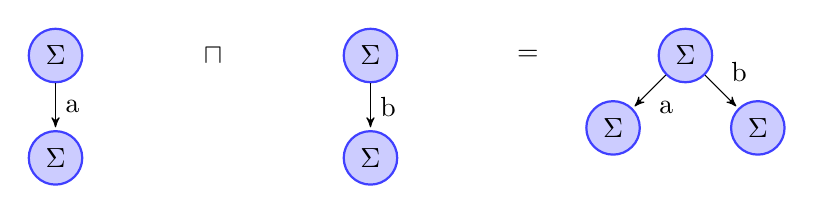
\begin{tikzpicture}[node distance=1.3cm,>=stealth',bend angle=45,auto]
  \tikzstyle{place}=[circle,thick,draw=blue!75,fill=blue!20,minimum size=6mm]
  \tikzstyle{red place}=[place,draw=red!75,fill=red!20]
  \tikzstyle{transition}=[rectangle,thick,draw=black!75,
  			  fill=black!20,minimum size=4mm]
  \tikzstyle{every label}=[red]
  \begin{scope}
    \node [place] (w1) {$\Sigma$};
    \node [place] (e1) [below of=w1] {$\Sigma$}
      edge [pre]  node[swap] {a}                 (w1);      
  \end{scope}
  \begin{scope}[xshift=4cm]
    \node [place] (w1) {$\Sigma$};
    \node [place] (e1) [below of=w1] {$\Sigma$}
      edge [pre]  node[swap] {b}                 (w1);      
  \end{scope} 
  \begin{scope}[xshift=8cm]
    \node [place] (w1) {$\Sigma$};
    \node [place] (e1) [below left of=w1] {$\Sigma$}
      edge [pre]  node[swap] {a}                 (w1);      
    \node [place] (e1) [below right of=w1] {$\Sigma$}
      edge [pre]  node[swap] {b}                 (w1);      
  \end{scope}
  \draw (2,0) node {$\sqcap$};
  \draw (6,0) node {$=$};
\end{tikzpicture}
\caption{Example of $\sqcap$.}
\end{figure}

\begin{figure}[H]
\centering
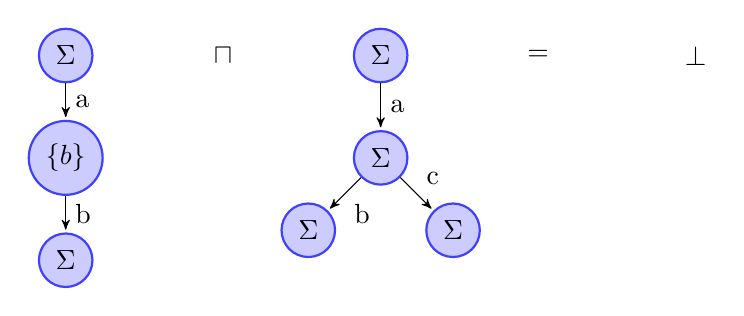
\begin{tikzpicture}[node distance=1.3cm,>=stealth',bend angle=45,auto]
  \tikzstyle{place}=[circle,thick,draw=blue!75,fill=blue!20,minimum size=6mm]
  \tikzstyle{red place}=[place,draw=red!75,fill=red!20]
  \tikzstyle{transition}=[rectangle,thick,draw=black!75,
  			  fill=black!20,minimum size=4mm]
  \tikzstyle{every label}=[red]
  \begin{scope}
    \node [place] (w1) {$\Sigma$};
    \node [place] (e1) [below of=w1] {$\{b\}$}
      edge [pre]  node[swap] {a}                 (w1);      
    \node [place] (e2) [below of=e1] {$\Sigma$}
      edge [pre]  node[swap] {b}                 (e1);      
  \end{scope}
  \begin{scope}[xshift=4cm]
    \node [place] (w1) {$\Sigma$};
    \node [place] (e1) [below of=w1] {$\Sigma$}
      edge [pre]  node[swap] {a}                 (w1);      
    \node [place] (e2) [below right of=e1] {$\Sigma$}
      edge [pre]  node[swap] {c}                 (e1);      
    \node [place] (e3) [below left of=e1] {$\Sigma$}
      edge [pre]  node[swap] {b}                 (e1);      
  \end{scope} 
  \begin{scope}[xshift=8cm]
    \node (w1) {$\bot$};
  \end{scope}
  \draw (2,0) node {$\sqcap$};
  \draw (6,0) node {$=$};
\end{tikzpicture}
\caption{Example of $\sqcap$.}
\end{figure}

\begin{figure}[H]
\centering
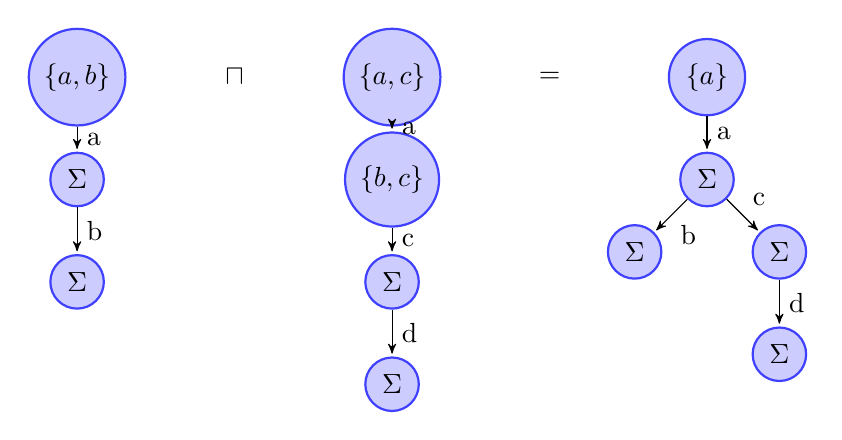
\begin{tikzpicture}[node distance=1.3cm,>=stealth',bend angle=45,auto]
  \tikzstyle{place}=[circle,thick,draw=blue!75,fill=blue!20,minimum size=6mm]
  \tikzstyle{red place}=[place,draw=red!75,fill=red!20]
  \tikzstyle{transition}=[rectangle,thick,draw=black!75,
  			  fill=black!20,minimum size=4mm]
  \tikzstyle{every label}=[red]
  \begin{scope}
    \node [place] (w1) {$\{a,b\}$};
    \node [place] (e1) [below of=w1] {$\Sigma$}
      edge [pre]  node[swap] {a}                 (w1);      
    \node [place] (e2) [below of=e1] {$\Sigma $}
      edge [pre]  node[swap] {b}                 (e1);      
  \end{scope}
  \begin{scope}[xshift=4cm]
    \node [place] (w1) {$\{a,c\}$};
    \node [place] (e1) [below of=w1] {$\{b,c\}$}
      edge [pre]  node[swap] {a}                 (w1);      
    \node [place] (e2) [below of=e1] {$\Sigma $}
      edge [pre]  node[swap] {c}                 (e1);      
    \node [place] (e3) [below of=e2] {$\Sigma $}
      edge [pre]  node[swap] {d}                 (e2);      
  \end{scope} 
  \begin{scope}[xshift=8cm]
    \node [place] (w1) {$\{a\}$};
    \node [place] (e1) [below of=w1] {$\Sigma $}
      edge [pre]  node[swap] {a}                 (w1);      
    \node [place] (e2) [below left of=e1] {$\Sigma $}
      edge [pre]  node[swap] {b}                 (e1);      
    \node [place] (e3) [below right of=e1] {$\Sigma $}
      edge [pre]  node[swap] {c}                 (e1);      
    \node [place] (e4) [below of=e3] {$\Sigma $}
      edge [pre]  node[swap] {d}                 (e3);      
  \end{scope}
  \draw (2,0) node {$\sqcap$};
  \draw (6,0) node {$=$};
\end{tikzpicture}
\caption{Example of $\sqcap$. \textbf{the label in the target of the $\TRANS{a}$ transition on the right is wrong?}}
\end{figure}

\begin{figure}[H]
\centering
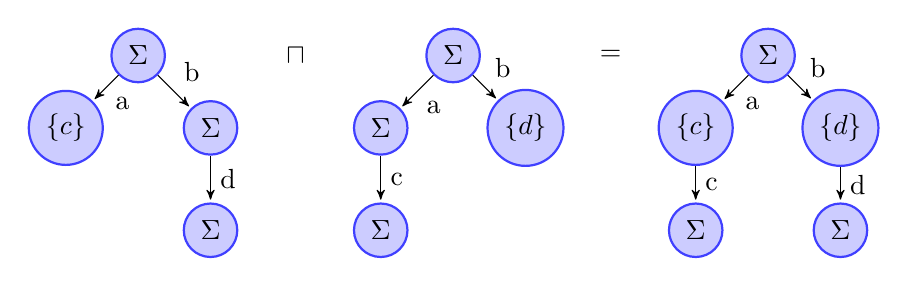
\begin{tikzpicture}[node distance=1.3cm,>=stealth',bend angle=45,auto]
  \tikzstyle{place}=[circle,thick,draw=blue!75,fill=blue!20,minimum size=6mm]
  \tikzstyle{red place}=[place,draw=red!75,fill=red!20]
  \tikzstyle{transition}=[rectangle,thick,draw=black!75,
  			  fill=black!20,minimum size=4mm]
  \tikzstyle{every label}=[red]
  
  \begin{scope}
    \node [place] (w1) {$\Sigma$};
    \node [place] (e1) [below left of=w1] {$\{c\}$}
      edge [pre]  node[swap] {a}                 (w1);      
    \node [place] (e2) [below right of=w1] {$\Sigma$}
      edge [pre]  node[swap] {b}                 (w1);      
    \node [place] (e3) [below of=e2] {$\Sigma$}
      edge [pre]  node[swap] {d}                 (e2);      
  \end{scope}
  
  \begin{scope}[xshift=4cm]
    \node [place] (w1) {$\Sigma$};
    \node [place] (e1) [below left of=w1] {$\Sigma$}
      edge [pre]  node[swap] {a}                 (w1);      
    \node [place] (e2) [below right of=w1] {$\{d\}$}
      edge [pre]  node[swap] {b}                 (w1);      
    \node [place] (e3) [below of=e1] {$\Sigma$}
      edge [pre]  node[swap] {c}                 (e1);      
  \end{scope}
  
  
  \begin{scope}[xshift=8cm]
    \node [place] (w1) {$\Sigma$};
    \node [place] (e1) [below left of=w1] {$\{c\}$}
      edge [pre]  node[swap] {a}                 (w1);      
    \node [place] (e2) [below right of=w1] {$\{d\}$}
      edge [pre]  node[swap] {b}                 (w1);      
    \node [place] (e3) [below of=e1] {$\Sigma$}
      edge [pre]  node[swap] {c}                 (e1);      
    \node [place] (e4) [below of=e2] {$\Sigma$}
      edge [pre]  node[swap] {d}                 (e2);      
  \end{scope}
  
  \draw (2,0) node {$\sqcap$};
  \draw (6,0) node {$=$};
\end{tikzpicture}
\caption{Example of $\sqcap$.}
\end{figure}


\begin{figure}[H]
\centering
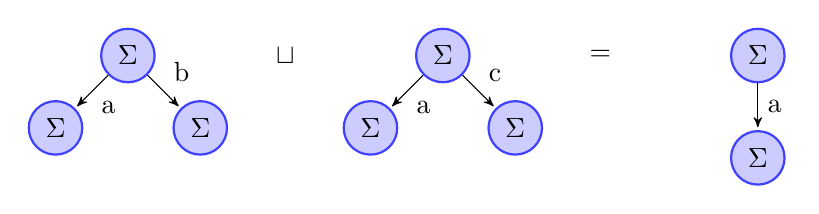
\begin{tikzpicture}[node distance=1.3cm,>=stealth',bend angle=45,auto]
  \tikzstyle{place}=[circle,thick,draw=blue!75,fill=blue!20,minimum size=6mm]
  \tikzstyle{red place}=[place,draw=red!75,fill=red!20]
  \tikzstyle{transition}=[rectangle,thick,draw=black!75,
  			  fill=black!20,minimum size=4mm]
  \tikzstyle{every label}=[red]
  \begin{scope}
    \node [place] (w1) {$\Sigma$};
    \node [place] (e1) [below left of=w1] {$\Sigma$}
      edge [pre]  node[swap] {a}                 (w1);      
    \node [place] (e2) [below right of=w1] {$\Sigma$}
      edge [pre]  node[swap] {b}                 (w1);      
  \end{scope}
  \begin{scope}[xshift=4cm]
    \node [place] (w1) {$\Sigma$};
    \node [place] (e1) [below left of=w1] {$\Sigma$}
      edge [pre]  node[swap] {a}                 (w1);      
    \node [place] (e2) [below right of=w1] {$\Sigma$}
      edge [pre]  node[swap] {c}                 (w1);      
  \end{scope}
  \begin{scope}[xshift=8cm]
    \node [place] (w1) {$\Sigma$};
    \node [place] (e1) [below of=w1] {$\Sigma$}
      edge [pre]  node[swap] {a}                 (w1);      
  \end{scope}
  \draw (2,0) node {$\sqcup$};
  \draw (6,0) node {$=$};
\end{tikzpicture}
\caption{Example of $\sqcup$}
\end{figure}

\begin{figure}[H]
\centering
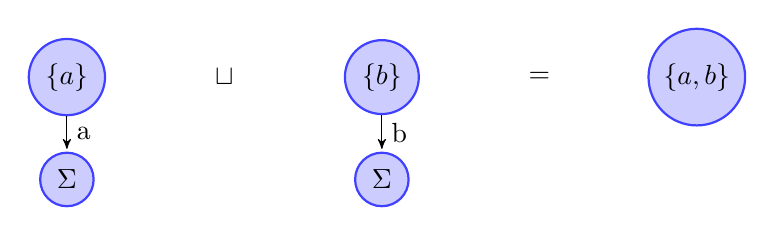
\begin{tikzpicture}[node distance=1.3cm,>=stealth',bend angle=45,auto]
  \tikzstyle{place}=[circle,thick,draw=blue!75,fill=blue!20,minimum size=6mm]
  \tikzstyle{red place}=[place,draw=red!75,fill=red!20]
  \tikzstyle{transition}=[rectangle,thick,draw=black!75,
  			  fill=black!20,minimum size=4mm]
  \tikzstyle{every label}=[red]
  \begin{scope}
    \node [place] (w1) {$\{a\}$};
    \node [place] (e1) [below of=w1] {$\Sigma$}
      edge [pre]  node[swap] {a}                 (w1);      
  \end{scope}
  \begin{scope}[xshift=4cm]
    \node [place] (w1) {$\{b\}$};
    \node [place] (e1) [below of=w1] {$\Sigma$}
      edge [pre]  node[swap] {b}                 (w1);      
  \end{scope}
  \begin{scope}[xshift=8cm]
    \node [place] (w1) {$\{a,b\}$};
  \end{scope}
  \draw (2,0) node {$\sqcup$};
  \draw (6,0) node {$=$};
\end{tikzpicture}
\caption{Example of $\sqcup$}
\end{figure}


\section{Computing Least Upper Bound ($\sqcup$)}

\begin{eqnarray*}
\MMM \sqcup \bot & = & \MMM \\
\bot \sqcup \MMM & = & \MMM \\
(\CAL{L},w) \sqcup (\CAL{L}',w') & = & \mathsf{lub}(\CAL{L}, \CAL{L}', (\MMM_\top, z), \{(w, w', z)\})
\end{eqnarray*}
where $\MMM_\top$ is the topmost model $(\mathcal{W}=\{z\}, \rightarrow=\{\}, \lambda=\{z \mapsto \Sigma\})$ for some state $z$.
$\mathsf{lub}$ takes four parameters: the two eremic transition systems $\CAL{L}$ and $\CAL{L}'$, an accumulator representing the constructed result so far, and a list of state triples (each triple contains one state from each of the two input models plus the state of the accumulated result) to consider next.
It is defined as:
\begin{eqnarray*}
\mathsf{lub}(\CAL{L}, \CAL{L}', \MMM, \{\}) & = & \MMM \\
\mathsf{lub}(\CAL{L}, \CAL{L}', ((\mathcal{W}, \rightarrow, \lambda), y), \{(w,w',x)\} \cup R) & = & \mathsf{lub}(\CAL{L}, \CAL{L}', ((\mathcal{W} \cup \mathcal{W}', \rightarrow \cup \rightarrow', \lambda'), y), R' \cup R\}
\end{eqnarray*}
where:
\begin{eqnarray*}
\{(a_i, w_i, w'_i) \;|\; i = 1 ... n\} & = & \mathsf{sharedT}((\CAL{L},w), (\CAL{L}',w')) \\
\mathcal{W}' & = & \{x_i \;|\; i = 1 ... n\} \\
\rightarrow' & = & \{(x, a_i, x_i) \;|\; i = 1 ... n\} \\
\lambda' & = & \lambda [x \mapsto \lambda(w) \cup \lambda(w)'] \\
R' & = & \{(w_i, w'_i, x_i) \;|\; i = 1 ... n\}
\end{eqnarray*}
Here, $\mathsf{sharedT}$ returns the shared transitions between two models, and is defined as:
\[
\mathsf{sharedT}(((\mathcal{W}, \rightarrow, \lambda),w) ((\mathcal{W}', \rightarrow', \lambda'),w')) =  \{(a, x, x') \;|\; w \xrightarrow{a} x \land w' \xrightarrow{a}' x'\}
\]
\begin{definition}
Let $Th(\MMM) =  \{\phi\ |\ \MMM \models \phi \}$.
\end{definition}

\begin{theorem}
\[
\MMM' \MODELLEQ \MMM
\qquad\text{iff}\qquad
Th(\MMM) \subseteq Th(\MMM') .
\]
\end{theorem}

\begin{proof}
\begin{case}
First, left to right
\end{case}
Assume $\MMM' \MODELLEQ \MMM$ and $\MMM \models \phi$.
We must show $\MMM' \models \phi$.
Let $\MMM = (\LLL, w)$ and $\MMM' = (\LLL', w')$.
The proof proceeds by induction on $\phi$.
The cases for $\top$ and $\land$ are trivial.

Assume $\phi = \MAY{a}\psi$ and assume  $(\LLL, w) \models  \MAY{a}\psi$.
Then $w \xrightarrow{a} x$ and $(\LLL, x) \models  \psi$.
As $\MMM'$ simulates $\MMM$, there is an $x'$ such that $(x,x') \in R$ and $w' \xrightarrow{a} x'$.
By the induction hypothesis, $(\LLL', x') \models \psi$.
Therefore, by the semantic clause for $!$, $(\LLL', w') \models  \MAY{a}\psi$.

Assume now that $\phi = \; ! \; A$, for some finite $A \subseteq \Sigma$, and that $(\LLL, w) \models \; ! \; A$.
By the semantic clause for $!$, $\lambda(w) \subseteq A$.
Since $(\LLL', w') \MODELLEQ (\LLL, w)$, by the definition of simulation of eremic transition systems, $\lambda(w) \supseteq \lambda'(w')$.
Therefore, $\lambda'(w') \subseteq \lambda(w) \subseteq A$.
Therefore, by the semantic clause for $!$, $(\LLL', w') \models  \; ! \; A$.

\begin{case}
Second, right to left.
\end{case}
Let $\MMM = (\LLL, w)$ and $\MMM' = (\LLL', w')$.
Assume $Th(\MMM) \subseteq Th(\MMM') $. We need to show that $\MMM'$ simulates $\MMM$.
In other words, we need to produce a relation $R \subseteq \mathcal{W} \times \mathcal{W}'$ where $(w,w') \in R$ and $R$ is a simulation from $(\LLL, w)$ to $ (\LLL', w')$.
Define $R = \{(x,x') \; | \; Th( (\LLL, x)) \subseteq Th( (\LLL', x'))\}$.
Clearly, $(w,w') \in R$, as $Th((\LLL, w)) \subseteq Th((\LLL', w')) $.
To show that $R$ is a simulation,  assume $x \xrightarrow{a} y$ in $\LLL$ and $(x,x') \in R$. We need to provide a $y'$ such that $x' \xrightarrow{a} y'$ in $\LLL'$.
Consider the formula $\MAY{a}\top$. Now $(\LLL, x) \models \MAY{a}\top$ because $x \xrightarrow{a} y$.
But as $(x,x') \in R$, $Th((\LLL, x)) \subseteq Th((\LLL', x')) $, so  $(\LLL', x') \models \MAY{a}\top$.
But, by the semantic clause for $\MAY{a}$, this means there is a $y'$ such that $x' \xrightarrow{a} y'$ in $\LLL'$,

Finally, we need to show that whenever $(x,x') \in R$, then $\lambda(x) \supseteq \lambda'(x')$.
Assume, first, that $\lambda(x)$ is finite. 
Then $(\LLL, x) \models \; ! \; \lambda(x)$.
But as $(x,x') \in R$, $Th((\LLL, x)) \subseteq Th((\LLL', x')) $, so  $(\LLL', x') \models \; ! \; \lambda(x)$.
But, by the semantic clause for $!$, $(\LLL', x') \models \; ! \; \lambda(x)$ iff $\lambda'(x') \subseteq \lambda(x)$.
Therefore $\lambda(x) \supseteq \lambda'(x')$.
If, on the other hand, $\lambda(x)$ is infinite, then $\lambda(x) = \Sigma$ (because the only infinite node labelling that we allow is $\Sigma$). Every node labelling is a subset of $\Sigma$, so in this case too, $\lambda(x) = \Sigma \supseteq \lambda'(x')$.


\end{proof}

\section{Core eremic logic: the EL$[\AND, !]$ fragment}

\subsection{Syntax}

\begin{definition} Given a set $\mathcal{S}$ of symbols, with $a$ ranging over
$\mathcal{S}$, and $A$ ranging over finite subsets of $\mathcal{S}$,
the formulae of EL$[\AND, !]$ are given by:

\begin{GRAMMAR}
  \phi 
     &\quad ::= \quad & 
  \top 
     \VERTICAL 
  \phi_1 \AND \phi_2  
     \VERTICAL 
  \MAY{a}{\phi}
     \VERTICAL 
  \fBang A 
\end{GRAMMAR}

\NI The $!$ operator is used to restrict the allowable transitions
coming out of a state.  Intuitively, $\fBang A$ means that the
\emph{only} transitions coming out of the current state are those
specified in $A$.
\end{definition}

\subsection{Semantics}

\begin{definition}
A {\bf model} is a triple $(\mathcal{W}, \rightarrow, \lambda)$,
containing a Labeled Transition System (a set of states $\mathcal{W}$,
and a transition relation $\rightarrow \; \subseteq \; \mathcal{W}
\times \mathcal{S} \times \mathcal{W}$), together with a
node-labelling $\lambda$ that maps each element of $\mathcal{W}$ to a
subset of $\mathcal{S}$.
\end{definition}
The intended interpretation is that $\lambda(w)$ is the set of allowed transition symbols emanating from $w$.
The $\lambda$ function is the semantic counterpart of the $!$ operator.

Now, for a model to be valid, we insist that the transitions coming out of a node $w$ are a subset of the allowed transitions in $\lambda(w)$:
\begin{definition}
A model $(\mathcal{W}, \rightarrow, \lambda)$ is {\bf valid} iff for all $w \in \mathcal{W}$, $ \{s \fOr \exists w' \; w \xrightarrow{s} w'\} \subseteq \lambda(w)$.
\end{definition}

\begin{definition}
A {\bf pointed model} is a pair $(l,w)$, where $m$ is a \emph{valid} model of the form $(\mathcal{W}, \rightarrow, \lambda)$, and $w$ is a distinguished state in $\mathcal{W}$.
\end{definition}
Formulae are interpreted in a pointed model $(l,w)$:
\begin{eqnarray}
(l,w) & \models & \top  \mbox{ always } \nonumber \\
(l,w) & \models & \phi_1 \AND \phi_2 \mbox{ iff } (l,w)  \models \phi_1 \mbox { and } (l,w) \models \phi_2 \nonumber \\
(l,w) & \models & \langle a \rangle \phi \mbox{ iff there is a } w \xrightarrow{a} w' \mbox { such that } (l,w') \models \phi \nonumber \\
(l,w) & \models & \fBang A \mbox{ iff } \lambda(w) \subseteq A\nonumber
\end{eqnarray}
Note that if a model is valid then $(l,w) \models \fBang A$ implies $\{s \fOr \exists w' \; w \xrightarrow{s} w'\} \subseteq A$.
From now on, we will restrict ourselves to valid models.

\begin{FIGURE}
\centering
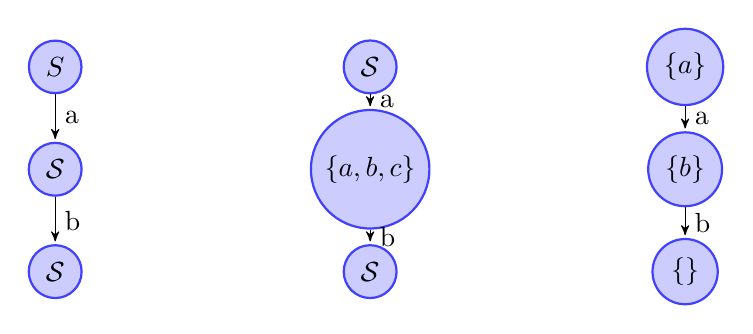
\begin{tikzpicture}[node distance=1.3cm,>=stealth',bend angle=45,auto]
  \tikzstyle{place}=[circle,thick,draw=blue!75,fill=blue!20,minimum size=6mm]
  \tikzstyle{red place}=[place,draw=red!75,fill=red!20]
  \tikzstyle{transition}=[rectangle,thick,draw=black!75,
  			  fill=black!20,minimum size=4mm]
  \tikzstyle{every label}=[red]
  \begin{scope}[xshift=0cm]
    \node [place] (w1) {$S$};
    \node [place] (e1) [below of=w1] {$\mathcal{S}$}
      edge [pre]  node[swap] {a}                 (w1);
    \node [place] (e2) [below of=e1] {$\mathcal{S}$}
      edge [pre]  node[swap] {b}                 (e1);
  \end{scope}   
  \begin{scope}[xshift=4cm]
    \node [place] (w1) {$\mathcal{S}$};
    \node [place] (e1) [below of=w1] {$\{a,b,c\}$}
      edge [pre]  node[swap] {a}                 (w1);
    \node [place] (e2) [below of=e1] {$\mathcal{S}$}
      edge [pre]  node[swap] {b}                 (e1);
  \end{scope}   
  \begin{scope}[xshift=8cm]
    \node [place] (w1) {$\{a\}$};
    \node [place] (e1) [below of=w1] {$\{b\}$}
      edge [pre]  node[swap] {a}                 (w1);
    \node [place] (e2) [below of=e1] {$\{\}$}
      edge [pre]  node[swap] {b}                 (e1);
  \end{scope}   
\end{tikzpicture}
\caption{Various models of $\langle a \rangle \langle b \rangle \top$}
\end{FIGURE}



\begin{FIGURE}
\begin{RULES}

  \ZEROPREMISERULENAMEDRIGHT
  {
    X \judge X
  }{Identity}
    \quad
  \ZEROPREMISERULENAMEDRIGHT
  {
    X \judge \top
  }{$\top$ Right}
    \quad
  \ZEROPREMISERULENAMEDRIGHT
  {
    \bot \judge X
  }{$\bot$ Left}
    \quad
  \TWOPREMISERULENAMEDRIGHT
  {
    X \judge Y
  }
  {
    Y \judge Z
  }
  {
    X \judge Z
  }{Transitivity}
    \\\\
  \ONEPREMISERULENAMEDRIGHT
  {
    X \judge Y
  }
  {
    X \AND Z \judge Y
  }{$\AND$ Left 1}
\end{RULES}
\caption{Proof rules. Put in remaining rules as they stabilise!}\label{figure:elAndBangRules}
\end{FIGURE}


\subsection{Inference Rules}

This section presend the inference rules for EL.
In EL, a judgement is of the form:

\[
  X \judge Y
\]

\NI Here, $X$ and $Y$ are \emph{single formulae}, not sequents.  To
avoid the need for structural inference rules, we restrict sequents to
single formulae on the left and right hand side. Figure
\ref{figure:elAndBangRules} presents all rules.  EL proof rules can be
grouped in two parts: standard rules and rules unique to EL.  Standard
rules are [\RULENAME{Identity}], [\RULENAME{$\top$-Right}],
[\RULENAME{$\bot$-Left}], [\RULENAME{Transitivity}],
[\RULENAME{$\AND$-Left 1}], [\RULENAME{$\AND$-Left 2}] and
[\RULENAME{$\AND$-Right}] hardly need explanation as they are variants
of familiar rules for propositional logic, see
e.g.~\cite{TroelstraAS:basprot,vanDalenD:logstr}.  We now explain the
rules that give EL's its distinctive properties: the relations betwen
$\langle \rangle$, $!$ and $\bot$.

The rule [\RULENAME{$\bot$-Right 1}] axiom captures the core
\emph{exclusion} property of !: for example if $A = \{male, female\}$
then $\MAY{orange}{X}$ is incompatible with $!A$. Thus $!A \AND
\MAY{orange}{X}$ must be false.

The rule [\RULENAME{$\bot$-Right 2}] expresses that falsity is 'global'
  and cannot be surpressed by prefixing. For example
  $\MAY{orange}{\bot}$ is false, simply because $\bot$ is already
  false.

Relatedly, the rule [\RULENAME{Transition Normal}] enables us to
prefix an inference with a may-modality. For example \martin{add good
  example here.}. Note that it is vital for soundness that $X$ in $X
\judge Y$ is a single formula. If we used transitional sequents $X_1, ..., X_n \judge Y$,
then the rule
\[
   \ONEPREMISERULE
   {
     X_1, ..., X_n \judge Y
   }
   {
     \MAY{a}{X_1}, ..., \MAY{a}{X_n} \judge \MAY{a}{Y}
   }
\]
is unsound. \martin{explain why, and why this is significant}. This
restriction is also in place in \cite{GaySJ:typcalosp} where a
Curry-Howard corrospondence between a fragment of linear logic
\cite{GirardJY:linlog,GirardJY:protyp} and a process calculus is
introduced. We discuss the relationship between EL and linear logic in
general, and linear logic's additive conjunction in Section
\ref{conclusion}.


The three rules [\RULENAME{!-Left}, \RULENAME{!-Right 1},
  \RULENAME{!-Right 2}] jointly express of the subset relation
$\subseteq$ on sets of symbols relates to provability. Readers
familiar with object-oriented programming will recognise
[\RULENAME{!-Left}] as contra-variant subtyping and [\RULENAME{!-Right
    1}] as covariant subtyping. Honda \cite{HondaK:thetypftpc}
develops a full theory of subtyping based on similar ideas.  All three
rules embody the intuition that whenever $A \subseteq A'$ then
asserting that $!A'$ is as strong as, or a stronger statement than
$!A$. [\RULENAME{!-Left}] simply states that we can always strengthen
our premise, while [\RULENAME{!-right 1}] allows us to weaken the
premise. \martin{add an intuitive explanation for [\RULENAME{!-right 2}]!}!

Note that the logic has no axioms. One reason for a purely rule-based
presentation is the absence of implication in the present fragment of
EL. \martin{explain in more detail!}

We close this subsection with a key meta-theorem.

\begin{theorem}\label{theorem:elAndBang:soundComplete}
The rules in Figure \ref{figure:elAndBangRules} are sound and complete:
\begin{enumerate}

\item\label{theorem:elAndBang:sound} (Soundness) $X \judge Y$ implies $X \models Y$.

\item\label{theorem:elAndBang:complete} (Completeness) $X \models Y$ implies $X \judge Y$.

\end{enumerate}
\end{theorem}

\NI Soundness is immediate from the definitions. Proof of completeness is
deferred to Section \ref{completenessProof}. 

\subsection{Example inferences}

We give some example inferences that illustrate how EL is used in
practise.
\martin{Add some example assertions here, for example some of those we
  use later.}

\subsection{Proof of completeness}\label{completenessProof}

\NI We now prove completeness of the rules in Figure
\ref{figure:elAndBangRules} (Theorem
\ref{theorem:elAndBang:soundComplete}.\ref{theorem:elAndBang:complete}).
The proof requires the development of additional technology which is
useful in other contexts as well.

\begin{itemize}

\item An ordering $\leq$ on models, which enables us to speak of the
  simplest model satisfying a formula.

\item An algorithm which gives the simplest model for a formula.

\item An algorithm which gives the a formula characterising a model.

\end{itemize}

\NI We now develop these three in turn and then prove completeness.

\subsubsection{A Partial Ordering on Pointed Models}

\NI We use the notion of simulation to define a partial ordering
$\leq$ on pointed models: \martin

\begin{definition}
$(l,w) \leq (l',w')$ if there is a simulation $Z$ from $l'$ to $l$ with $(w',w) \in Z$
\end{definition}
Intuitively, $m \leq n$ if $m$ can match all the transitions of $n$ while respecting the transitions-restrictions.

To make our models into a lattice, we add a bottom element $\bot$ and stipulate that $\bot \leq m$ for all pointed models $m$.
The topmost element in the lattice is the pointed model $( (\{w\}, \{\}, \{w \mapsto \mathcal{S}\}), w)$ (for some state $w$): this is the model with no transitions and no transition restrictions.

\subsubsection{Defining $\mu$ - the Simplest Pointed Model Satisfying a Formula}
We define a function $\mu$ which, given a formula $\phi$, produces the simplest\footnote{``Simplest'' as in the least upper bound, according to $\leq$, defined in formulae of simulation.} model which satisfies $\phi$:
\begin{eqnarray}
\mu (\top) & = & ( (\{v\}, \{\}, \{v \mapsto \mathcal{S}\}), v) \nonumber \\
\mu (\fBang A) & = & ( (\{v\}, \{\}, \{v \mapsto A\}), v) \nonumber \\
\mu (\phi_1 \AND \phi_2) & = & \mu(\phi_1) \sqcap \mu(\phi_2) \nonumber \\
\mu (\langle a \rangle \phi) & = & ( (\mathcal{W} \cup \{w'\}, \rightarrow \cup (w' \xrightarrow{a} w), \lambda \cup \{w' \mapsto \mathcal{S}\}]), w') \nonumber \\
		& & \mbox{where }\mu(\phi) = ( (\mathcal{W}, \rightarrow, \lambda), w) \nonumber \\
		& & \mbox{and }w' \mbox{ is a new state not appearing in }\mathcal{W} \nonumber
\end{eqnarray}
The only complex case is the clause for $\mu (\phi_1 \AND \phi_2)$, which uses the $\sqcap$ function, defined as\footnote{We assume that the sets of states in the two pointed models are disjoint.}:

\begin{eqnarray*}
  \bot \sqcap X 
     & = & 
  \bot \nonumber 
     \\
  X \sqcap \bot 
     & = & 
  \bot \nonumber 
     \\
  m \sqcap n 
     & = & 
  \begin{cases}
    \mathsf{merge}(m, n) & \text{if}\ \mathsf{consistent}(m, n) \\
    \bot & \text{else}
  \end{cases}
\end{eqnarray*}

\noindent The $\mathsf{consistent}$ predicate is true of pointed models $m$ and $n$ if the out-transitions on $m$'s root node respect the labelling on $n$'s root node, and the out-transitions on $n$'s root node respect the labelling on $m$'s root node. In other words:
\begin{eqnarray}
\mathsf{consistent}(m, n) & \mbox{ iff } & \mathsf{out}(m) \subseteq \mathsf{restriction}(n) \mbox{ and} \nonumber \\
& & \mathsf{out}(n) \subseteq \mathsf{restriction}(m) \nonumber
\end{eqnarray}
where:
\begin{eqnarray}
\mathsf{out}(((\mathcal{W},\rightarrow,\lambda),w)) & = & \{ s \fOr \exists x . w \xrightarrow{s} x \} \nonumber \\
\mathsf{restriction}(((\mathcal{W},\rightarrow,\lambda),w)) & = & \lambda(w) \nonumber
\end{eqnarray}
Now the $\mathsf{merge}$ function fuses two pointed models together:
\[
\mathsf{merge}( ( (\mathcal{W}, \rightarrow, \lambda), w),  ( (\mathcal{W}', \rightarrow', \lambda'), w')) = ((\mathcal{W} \cup \mathcal{W}', \rightarrow \cup \rightarrow'_2, \lambda_2 \cup \lambda'_2), w)
\]
where:
\begin{eqnarray}
\rightarrow'_2 & = & \rightarrow' \mbox{ with } w' \mbox{ replaced by } w \nonumber \\
\lambda_2 & = & \lambda \mbox{ with } w \mapsto \lambda(w) \cap \lambda'(w') \nonumber \\
\lambda'_2 & = & \lambda' \mbox{ with } w' \mbox{ removed } \nonumber
\end{eqnarray}
It is easy to show that $\mu$ satisfies the following propositions:
\begin{eqnarray}
\mu(\phi) & \models & \phi \nonumber \\
\mbox{if }n \models \phi \mbox{ and } m \leq n & \mbox{ then } & m \models \phi \nonumber
\end{eqnarray}

\subsubsection{Defining $\theta$ - a Formula that Characterises a Model}
The inverse function $\theta$ produces a formula that characterises a given pointed model:
\begin{eqnarray}
\theta(\bot) & = & \langle a \rangle \top \AND ! \{ \} \mbox{ for some symbol }a \nonumber \\
\theta(l, w) & = & \mathsf{bang}(l,w) \AND \bigwedge_{(s,w') \in \mathsf{trans}(l,w)} \langle s \rangle \theta(l, w') \nonumber 
\end{eqnarray}
Here:
\begin{eqnarray}
\mathsf{bang}((\mathcal{W},\rightarrow,\lambda),w) & = & \top \mbox{ if } \lambda(w) = \mathcal{S} \nonumber \\
\mathsf{bang}((\mathcal{W},\rightarrow,\lambda),w) & = & ! \; \lambda(w) \mbox{ otherwise } \nonumber \\
\mathsf{trans}((\mathcal{W},\rightarrow, \lambda),w) & = & \{(s,w') | w \xrightarrow{s} w' \} \nonumber
\end{eqnarray}
Note that $\theta(m)$ is finite if $m$ contains no cycles and if $\lambda(x)$ is either $\mathcal{S}$ or finite for all states $x$.
Note also that $\mu$ and $\theta$ are inverses of each other in that:
\begin{eqnarray}
\mu(\theta(m)) & = & m \nonumber \\
\theta(\mu(p)) & \mbox{ iff } & p \nonumber
\end{eqnarray}


We will show that $p \models q$ implies there is a derivation of $p
\judge q$.  Our proof will make use of two lemmas:
\begin{itemize}
\item
Lemma 4: if $m \models p$ then $\theta(m) \judge p$.
\item
Lemma 5: for all formulae $p$, $p \judge \theta(\mu(p))$.
\end{itemize}
With these two lemmas in hand, the proof is straightforward.
\begin{theorem}
If $p \models q$ then $p \judge q$
\end{theorem}
\begin{proof}
Assume $p \models q$. 
Then all models which satisfy $p$ also satisfy $q$.
In particular, $\mu(p) \models q$.
Then $\theta(\mu(p)) \judge q$ by Lemma 1.
But we also have, by Lemma 2, $p \judge \theta(\mu(p)) $.
So by transitivity, we have $p \judge q$.
\qed
\end{proof}
Next we will prove Lemma 4.
\begin{lemma}
If $m \models p$ then $\theta(m) \judge p$.
\end{lemma}
\begin{proof}
Induction on $p$.
\setcounter{mycase}{0}

\begin{mycase}
$p$ is $\top$
\end{mycase}
Then we can prove  $\theta(m) \judge p$ immediately using axiom {\bf $\top$ Right}.

\begin{mycase}
$p$ is $q \AND q'$
\end{mycase}
By the induction hypothesis, $\theta(m) \judge q$ and $\theta(m) \judge q'$.
The proof of $\theta(m) \judge q \AND q'$ follows immediately using {\bf $\AND$ Right}.

\begin{mycase}
$p$ is $\langle a \rangle q$
\end{mycase}
If $m \models \langle a \rangle q$, then either $m = \bot$ or $m$ is a pointed model of the form $(l,w)$.
\begin{subcase}
$m = \bot$
\end{subcase}
In this case, $\theta(m) = \theta(\bot) = \bot$. (Recall, that we are overloading $\bot$ to mean both the pointed model at the bottom of our lattice and a formula (such as $\langle s \rangle \top \AND !\{\}$) which is always false).
In this case, $ \theta(\bot) \judge  \langle a \rangle q$ using {\bf $\bot$ Left}.

\begin{subcase}
 $m$ is a pointed model of the form $(l,w)$
 \end{subcase}
Given $m \models \langle a \rangle q$, and that $m$ is a pointed model of the form $(l,w)$, we know that:
\[
(l,w) \models \langle a \rangle q
\]
From the satisfaction clause for $\langle a \rangle$, it follows that:
\[
\exists w' \mbox{ such that } w \xrightarrow{a} w' \mbox { and } (l,w') \models q
\]
By the induction hypothesis:
\[
\theta( (l,w') ) \judge q
\]
Now by {\bf Transition Normal}:
\[
\langle a \rangle \theta( (l,w') ) \judge \langle a \rangle q
\]
Using repeated application of {\bf $\AND$ Left}, we can show:
\[
\theta((l,w)) \judge \langle a \rangle \theta((l,w'))
\]
Finally, using {\bf Transitivity}, we derive:
\[
\theta((l,w)) \judge  \langle a \rangle q
\]
\begin{mycase}
$p$ is $\fBang q$
\end{mycase}
If $(l,w) \models \fBang A$, then $\lambda(w) \subseteq A$.
Then $\theta(l,w) = ! \; \lambda(w) \AND \phi$.
Now we can prove $! \; \lambda(w) \AND \phi \judge \fBang A$ using  {\bf $!$ Right 1} and repeated applications of {\bf $\AND$ Left}.
\qed
\end{proof}

\begin{lemma}
For all formulae $p$, we can derive $p \judge \theta(\mu(p))$.
\end{lemma}
Explanation: $\mu(p)$ is the simplest model satisfying $p$, and $\theta(m)$ is the simplest formula describing $m$, so $\theta(\mu(p))$ is a simplified form of $p$. This lemma states that EL has the inferential capacity to transform any proposition into its simplified form.
\begin{proof}
Induction on $p$.

\setcounter{mycase}{0}

\begin{mycase}
$p$ is $\top$
\end{mycase}
Then we can prove  $\top \judge \top$ using either {\bf $\top$ Right} or {\bf Identity}.

\begin{mycase}
$p$ is $q \AND q'$
\end{mycase}
By the induction hypothesis, $q \judge \theta(\mu(q))$ and $q' \judge \theta(\mu(q'))$.
Using {\bf $\AND$ Left} and {\bf $\AND$ Right}, we can show:
\[
q \AND q' \judge \theta(\mu(q)) \AND \theta(\mu(q'))
\]
Lemma 6, proven below, states that, for all models $m$ and $n$:
\[
\theta(m) \AND \theta(n) \judge \theta (m \sqcap n)
\]
From Lemma 6 (substituting $\mu(q)$ for $m$ and $\mu(q')$ for $n$), it follows that:
\[
\theta(\mu(q)) \AND \theta(\mu(q')) \judge \theta(\mu(q \AND q'))
\]
Our desired result follows using {\bf Transitivity}.

\begin{mycase}
$p$ is $\langle a \rangle q$
\end{mycase}
By the induction hypothesis, $q \judge \theta(\mu(q))$.
Now there are two sub-cases to consider, depending on whether or not $\theta(\mu(q)) = \bot$.
\begin{subcase}
$\theta(\mu(q)) = \bot$
\end{subcase}
In this case, $\theta(\mu(\langle a \rangle q))$ also equals $\bot$. 
By the induction hypothesis:
\[
q \judge \bot
\]
By {\bf Transition Normal}:
\[
\langle a \rangle q \judge \langle a \rangle \bot
\]
By {\bf Bottom Right 2}:
\[
\langle a \rangle \bot \judge \bot
\]
The desired proof that:
\[
\langle a \rangle q \judge \bot
\]
follows by {\bf Transitivity}.
\begin{subcase}
$\theta(\mu(q)) \neq \bot$
\end{subcase}
By the induction hypothesis, $q \judge \theta(\mu(q))$.
So, by {\bf Transition Normal}:
\[
\langle a \rangle q \judge \langle a \rangle \theta(\mu(q))
\]
The desired conclusion follows from noting that:
\[
 \langle a \rangle \theta(\mu(q)) = \theta(\mu(\langle a \rangle q))
 \]
 \begin{mycase}
$p$ is $\fBang A$
\end{mycase}
If $p$ is $\fBang A$, then $ \theta(\mu(p))$ is $\fBang A \AND \top$.
We can prove $\fBang A \judge \fBang A \AND \top$ using {\bf $\AND$ Right}, {\bf $\top$ Right} and {\bf Identity}.
\qed
\end{proof}
Finally, to fill the hole in Case 2 above, we need to show that:
\begin{lemma}
For all models $m$ and $n$, $\theta(m) \AND \theta(n) \judge \theta (m \sqcap n)$.
\end{lemma}

\begin{proof}

There are two cases to consider, depending on whether or not $(m \sqcap n) = \bot$.

\setcounter{mycase}{0}

\begin{mycase}
$(m \sqcap n) = \bot$
\end{mycase}
If $(m \sqcap n) = \bot$, there are three possibilities:
\begin{itemize}
\item
$m = \bot$
\item
$n = \bot$
\item
Neither $m$ nor $n$ are $\bot$, but together they are incompatible. 
\end{itemize}
If either $m$ or $n$ is $\bot$, then the proof is a simple application of {\bf Identity} followed by {\bf $\AND$ Left}.

Next, let us consider the case where neither $m$ nor $n$ are $\bot$, but together they are incompatible.
Let $m$ be the pointed model $(l, w)$ and let $n$ be $(l', w')$.
If $(l, w) \sqcap (l', w') = \bot$, then\footnote{The alternative, in which the $s$-transition is in $n$ and the transition-restriction is in $m$, is identical, swapping $m$ with $n$.} there exists a symbol $s$ and a state $w_2$ such that $w \xrightarrow{s} w_2$ but $s \notin \lambda'(w')$.

In this case, by the definition of $\theta$, $\theta(m) \judge \langle s \rangle \top$, using  {\bf Identity} and repeated applications of {\bf $\AND$ Left}.
Further, by the definition of $\theta$, $\theta(n) \judge \; ! \; \lambda'(w')$, using  {\bf Identity} and repeated applications of by {\bf $\AND$ Left}. Again, $s \notin  \lambda'(w')$.

Therefore,  $\theta(m) \AND \theta(n) \judge \bot$, using  {\bf $\AND$ Right} and  {\bf Bottom Right 1}.
\begin{mycase}
$(m \sqcap n) \neq \bot$
\end{mycase}
In this case, let $(l,w) = m$ and let $(l',w')=n$.
Then, from the definition of $\mathsf{merge}$ above:
\[
\theta((l,w) \sqcap (l',w')) = \; ! \; (\lambda(w) \cap \lambda'(w')) \AND \bigwedge_{w \xrightarrow{s} w_2} \langle s \rangle \theta((l, w_2)) \AND \bigwedge_{w' \xrightarrow{s} w_3} \langle s \rangle \theta((l', w_3))
\]
We need to show that $\theta((l,w)) \AND \theta((l',w')) \judge \theta((l,w) \sqcap (l',w'))$ - or in other words, that:
\begin{itemize}
\item
$\theta((l,w)) \AND \theta((l',w')) \judge \; ! \; (\lambda(w) \cap \lambda'(w'))$
\item
$\theta((l,w)) \AND \theta((l',w')) \judge \langle s \rangle \theta((l, w_2))$ for all $s,w_2$ such that $w \xrightarrow{s} w_2$
\item
$\theta((l,w)) \AND \theta((l',w')) \judge \langle s \rangle \theta((l, w_3))$ for all $s,w_3$ such that $w' \xrightarrow{s} w_3$
\end{itemize}
To show $\theta((l,w)) \AND \theta((l',w')) \judge \; ! \; (\lambda(w) \cap \lambda'(w'))$, note that $\theta((l,w))  \judge \; ! \; \lambda(w)$ and $\theta((l',w')) \judge \; ! \;  \lambda'(w'))$.
We can derive $\theta((l,w)) \AND \theta((l',w')) \judge \; ! \; (\lambda(w) \cap \lambda'(w'))$ using {\bf $\AND$ Right} and {\bf $!$ Right 2}. 

To show $\theta((l,w)) \AND \theta((l',w')) \judge \langle s \rangle \theta((l, w_2))$, observe from the definition of $\theta$ that $\theta((l,w))$ contains a conjunct $\langle s \rangle \theta((l, w_2))$, so the proof follows from  {\bf $\AND$ Right} and repeated applications of  {\bf $\AND$ Left}. The same procedure applies to show $\theta((l,w)) \AND \theta((l',w')) \judge \langle s \rangle \theta((l, w_3))$ for all $s,w_3$ such that $w' \xrightarrow{s} w_3$.

This completes Lemma 6 and hence the Completeness Proof.
\qed

\end{proof}

\subsection{The standard translation from  EL into FOL}

We will translate EL into a restricted fragment of FOL.
There are three types of predicate:
\begin{itemize}
\item
A 0-place predicate $\top$, which is true in all models.
\item
A set of two-place predicates $Arr_s(x, y)$, one for each $s \in \mathcal{S}$, where $x$ and $y$ are of type $State$. $Arr_s(x, y)$ is true if $x \xrightarrow{s} y$.
\item
A set of one-place predicates $Restrict_A$, one for each finite subset $A \subseteq \mathcal{S}$. 
$Restrict_{A}(x)$ is true if $\lambda(x) = A$.
\end{itemize}
With $x_1, x_2$ being state variables, $s$ a symbol in $\mathcal{S}$, and $A$ ranging over subsets of $\mathcal{S}$, our restricted fragment of FOL has formulae of the form:
\begin{GRAMMAR}
  \phi 
     &\quad ::= \quad&
  \top \fOr Arr_{s}(x_1, x_2)\fOr Restrict_A(x_1) \fOr \phi_1 \AND \phi_2 \fOr \exists x_1 . \phi 
\end{GRAMMAR}
Notice that this fragment of FOL has no negation, disjunction, implication, or universal quantification.

The translation of an EL formula is relative to a variable $x$ (which will be instantiated to the particular state at which we are evaluating the formula):
\begin{eqnarray}
T_x(\top) & = & \top \nonumber \\
T_x(\phi_1 \AND \phi_2) & = & T_x(\phi_1) \AND T_x(\phi_2) \nonumber \\
T_x(\langle s \rangle \phi) & = & \exists y \; . \; Arr_s(x,y) \AND T_y(\phi) \nonumber \\
T_x(\fBang A) & = & Restrict_A(x) \nonumber
\end{eqnarray}
So, for example:
\[
T_x(\langle a \rangle \top \AND \fBang \{a\}) = \exists y \; . \; Arr_a(x,y) \AND \top \AND Restrict_{\{a\}}(x)
\]


\subsection{Compactness}


\section{A decision procedure for eremic logic}\label{decisionprocedure}

In Section \ref{coreEL} we presented \ELABR{} and established the key
properties of completeness and compactness.  Here we give a
linear-time decision procedure.  The linear time-complexity of the
decision procedure is an indication that \ELABR{} can be useful as a
query language in knowledge representation. 

\NI Since \ELABR{} has no connectives for disjunction or implication, its
decision procedure is straightforward and efficient.  Although there
are an infinite number of models which satisfy any expression, the
satisfying models form a lattice with a least upper bound.  The $\SIMPL$
function defined above gives us the minimal model satisfying an
expression.  Using this least upper bound, we can calculate entailment
by checking a \emph{single model}.  To decide whether $p \models q$,
we use the following theorem:

\begin{theorem}\label{theorem:decision}
  The following are equivalent:
  \begin{enumerate}
    \item\label{theorem:decision:1} For all eremic models $\MMM$,
      $\MMM \models \phi$ implies $\MMM \models \psi$.
    \item\label{theorem:decision:2} $\SIMPL{\phi} \models \psi$.
  \end{enumerate}
\end{theorem}

\begin{proof}
The implication from  (\ref{theorem:decision:1}) to
(\ref{theorem:decision:2}) is trivial because $\SIMPL{\phi}$ is a model by construction.

For the reverse direction, assume $\MMM \models \phi$. We need to show
$\MMM \models \psi$.  Now if $\MMM \models \phi$ then $\MMM \MODELLEQ
\SIMPL{\phi}$ (by Lemma \ref{...}).  Further, if $\MMM' \models \xi $
and $\MMM \MODELLEQ \MMM'$ then $\MMM \models \xi $ by Theorem
\ref{completeLattice}. So, substituting $\psi$ for $\xi $ and
$\SIMPL{\phi}$ for $\MMM'$, it follows that $\MMM \models \psi$.
\end{proof}

\NI Given this theorem, the decision procedure is straightforward: to
test if $\phi \models \psi$, we construct $\SIMPL{\phi}$, and then inspect whether
$\SIMPL{\phi} \models \psi$.  Construction of $\SIMPL{\phi}$ is linear in the size of
$\phi$, and computing whether a model satisfies $\psi$ is linear in the size
of $\psi$, so computing whether $\phi \models \psi$ is $O(|\phi|+|\psi|)$.

\martin{Can we say more about the decision procedure? Example? Talk
  about Haskell code?}


\subsection{Incompatibility semantics}\label{incompatibility}

\NI Define the set of formulae\footnote{Brandom \cite{brandom} defines
  incompatibility slightly differently: he defines the set of
  \emph{sets} of formulae which are incompatible with a \emph{set} of
  formulae.  But in EL, if a set of formulae is incompatible, then
  there is an incompatible subset of that set with exactly two
  members.  So we can work with the simpler definition in the text
  above.}  incompatible with $\phi$ as:
\[
\mathcal{I}(\phi) = \{ \psi \; | \; \SIMPL{\phi} \sqcap \SIMPL{\psi} = \bot \}
\]
EL satisfies Robert Brandom's \textbf{incompatibility semantics}  property:
\[
\phi \models \psi \; \mbox{ iff } \; \mathcal{I}(\psi) \subseteq \mathcal{I}(\phi)
\]
Before proving this, I want to say something about why satisfying this incompatibility semantics property is important.
Not all logics satisfy this property. 
Brandom has shown that First Order Logic and S5 satisfy the incompatibility semantics property, but it is an open question which other logics satisfy it.
HML satisfies it, but HML without negation does not.
EL is the \emph{simplest logic we have found} that satisfies the property.

To prove this, we need to first define a related incompatibility function on  models.
$\mathcal{J}(\MMM)$ is the set of models that are incompatible with $\MMM$:
\[
\mathcal{J}(\MMM) = \{ \MMM_2 \; | \; \MMM \sqcap \MMM_2 = \bot \}
\]
We shall make use of three lemmas:
\begin{lemma}
\label{inc1}
$\mbox{if }\phi \models \psi \mbox{ then } \SIMPL{\phi} \MODELLEQ \SIMPL{\psi}$
\end{lemma}
\begin{lemma}
\label{inc2}
$\mbox{if }\MMM \MODELLEQ \MMM_2 \mbox{ then } \MMM_3 \sqcap \MMM \MODELLEQ \MMM_3 \sqcap \MMM_2$
\end{lemma}
\begin{lemma}
\label{inc3}
$\mbox{if }\mathcal{I}(\psi) \subseteq \mathcal{I}(\phi) \mbox{ then } \mathcal{J}(\SIMPL{\psi}) \subseteq \mathcal{J}(\SIMPL{\phi})$
\end{lemma}

\begin{theorem}
$\phi \models \psi \; \mbox{ iff } \; \mathcal{I}(\psi) \subseteq \mathcal{I}(\phi)$
\end{theorem}

\begin{proof}

Left to right: Assume $\phi \models \psi$ and $\xi \in \mathcal{I}(\psi)$.  By
Lemma \ref{inc1}, $\SIMPL{\phi} \MODELLEQ \SIMPL{\psi}$.  From $\xi \in \mathcal{I}(\psi)$,
$\SIMPL{\xi} \sqcap \SIMPL{\psi} = \bot$.  By Lemma \ref{inc2}, $\SIMPL{\xi} \sqcap
\SIMPL{\phi} \MODELLEQ \SIMPL{\xi} \sqcap \SIMPL{\psi}$ (substituting $\SIMPL{\xi}$
for $x$, $\SIMPL{\phi}$ for $m$, and $\SIMPL{\psi}$ for $n$).  But if
$\SIMPL{\xi} \sqcap \SIMPL{\psi} = \bot$, and $\SIMPL{\xi} \sqcap \SIMPL{\phi}
\MODELLEQ \SIMPL{\xi} \sqcap \SIMPL{\psi}$, then $\SIMPL{\xi} \sqcap \SIMPL{\phi} =
\bot$ also, because the only element that is $\MODELLEQ \bot$ is $\bot$
itself.  But if $\SIMPL{\xi} \sqcap \SIMPL{\phi} = \bot$, then $\xi \in
\mathcal{I}(\phi)$.  \qed

Right to left: assume, for reductio, that $\MMM \models \phi$ and $\MMM \nvDash
\psi$. we will show that $\mathcal{I}(\psi) \nsubseteq \mathcal{I}(\phi)$.
Assume $\MMM \models \phi \mbox{ and } \MMM \nvDash \psi$. We will construct
another model $\MMM_2$ such that $\MMM_2 \in \mathcal{J}(\SIMPL{\psi})$ but $\MMM_2
\notin \mathcal{J}(\SIMPL{\phi})$.  This will entail, via Lemma \ref{inc3}, that
$\mathcal{I}(\psi) \nsubseteq \mathcal{I}(\phi)$.

If $\MMM \nvDash \psi$, then there is a formula $\psi'$ that does not contain
$\AND$ such that $\psi \models \psi'$ and $\MMM \nvDash \psi'$. $\psi'$ must be
either of the form (i) $\langle a_1 \rangle ... \langle a_n \rangle
\top$ (for $n > 0$) or (ii) of the form $\langle a_1 \rangle
... \langle a_n \rangle \; !\{A\}$ where $A \subseteq \mathcal{S}
\mbox{ and } n >= 0$.

In case (i), there must be an $i$ between $0$ and $n$ such that $\MMM
\models \langle a_1 \rangle ... \langle a_i \rangle \top$ but $\MMM
\nvDash \langle a_1 \rangle ... \langle a_{i+1} \rangle \top$. We need
to construct another model $\MMM_2$ such that $\MMM_2 \sqcap \SIMPL{\psi} = \bot$,
but $\MMM_2 \sqcap \SIMPL{\phi} \neq \bot$. Letting $\MMM =
((\mathcal{W},\rightarrow,\lambda),w)$, then $\MMM \models \langle a_1
\rangle ... \langle a_i \rangle \top$ implies that there is at least
one sequence of states of the form $w, w_1, ..., w_i$ such that $w
\xrightarrow{a_1} w_1 \rightarrow ... \xrightarrow{a_i} w_i$.  Now let
$\MMM_2$ be just like $\MMM$ but with additional transition-restrictions on
each $w_i$ that it not include $a_{i+1}$.  In other words,
$\lambda_{\MMM_2}(w_i) = \lambda_\MMM(w_i) - \{a_{i+1}\}$ for all $w_i$ in
sequences of the form $w \xrightarrow{a_1} w_1 \rightarrow
... \xrightarrow{a_i} w_i$. Now $\MMM_2 \sqcap \SIMPL{\psi} = \bot$ because of
the additional transition restriction we added to $\MMM_2$, which rules out
$\langle a_1 \rangle ... \langle a_{i+1} \rangle \top$, and
a-forteriori $\psi$. But $\MMM_2 \sqcap \SIMPL{\phi} \neq \bot$, because $\MMM
\models \phi$ and $\MMM_2 \MODELLEQ \MMM$ together imply $\MMM_2 \models \phi$. So $\MMM_2$ is
indeed the model we were looking for, that is incompatible with
$\SIMPL{\psi}$ while being compatible with $\SIMPL{\phi}$.

In case (ii), $\MMM \models \langle a_1 \rangle ... \langle a_n \rangle
\top$ but $\MMM \nvDash \langle a_1 \rangle ... \langle a_n \rangle !A$
for some $A \subset \mathcal{S}$. We need to produce a model $\MMM_2$ that
is incompatible with $\SIMPL{\psi}$ but not with $\SIMPL{\phi}$. Given that
$\MMM \models \langle a_1 \rangle ... \langle a_n \rangle \top$, there is
a sequence of states $w, w_1, ..., w_n$ such that $w \xrightarrow{a_1}
w_1 \rightarrow ... \xrightarrow{a_i} w_n$. Let $\MMM_2$ be the model just
like $\MMM$ except it has an additional transition from each such $w_n$
with a symbol $a \notin A$. 
Clearly, $\MMM_2 \sqcap \SIMPL{\psi'} = \bot$
because of the additional $a$-transition, and given that $\psi \models
\psi'$, it follows that $\MMM_2 \sqcap \SIMPL{\psi} = \bot$. Also, $\MMM_2 \sqcap
\SIMPL{\phi} \neq \bot$, because $\MMM_2 \MODELLEQ \MMM$ and $\MMM \models \phi$.


\end{proof}

\section{Eremic logic and negation}

Our motivation for investigating eremic logic has been to give an
alternative account of negation, based on the concept of exclusion.
In this section we study how to recover negation in eremic logic. For
this purpose, we enrich eremic logic with negation as well as
disjunction, and show how negation can be explained in terms of plain
eremic logic with disjunction. We then discuss the meaning of excluded
middle in eremic logic.

\begin{definition}
Given a set $\Sigma$ of symbols, the \emph{formulae of eremic logic
  with negation}, collectively denoted EL$[\land, !, \neg]$, are given
by the following grammar.

\begin{GRAMMAR}
  \phi 
     &\quad ::= \quad & 
   \top \fOr \bot \fOr \neg \phi \fOr \phi \land \psi \fOr \langle a \rangle \phi \fOr \fBang A 
\end{GRAMMAR}

\NI We can now define disjunction $\phi \lor \psi$ and implication
$\phi \IMPLIES \psi$ by de Morgan duality: $\phi \OR \psi$ is short
for $\neg (\neg \phi \land \neg \psi )$, and $\phi \IMPLIES \psi$  abbreviates
$\neg\phi \OR \psi$.
\end{definition}

The semantics of EL$[\land, !, \neg]$ is just as in EL$[\land, !]$
above, except for the obvious clauses for negation and disjunction:
\begin{eqnarray*}
\MMM \models \neg \phi &\quad\mbox{ iff }\quad& \MMM \nvDash \phi  
%\MMM \models \phi \lor \psi &\mbox{ iff }& \MMM \models \phi \text{ or }   \MMM \models \psi
\end{eqnarray*}

\martin{Can we say something about the proof rules for EL$[\land, !, \neg]$?}

Negation is a core operation of classical logic, and its absence makes
eremic logic unusual. In order to understand eremic logic better, we
now investigate how negation can be seen as a definable abbreviation
in eremic logic with disjunction. The key idea is that 
\[
   \neg \MAY{a}{\phi}
\]
can be false in two ways: there is no $a$-labelled action at the
current state, or there is, but $\phi$ is false. Both arms of this
disjunction can be expressed in eremic logic:

\begin{itemize}

\item $!\Sigma \setminus \{a\}$.

\item $\MAY{a}{\neg \phi}$.

\end{itemize}

\NI Hence, we can see $\neg \MAY{a}{\phi}$ as a shorthand for 
\[
   \Sigma \setminus \{a\} \OR \MAY{a}{\neg \phi}
\]

\NI Negation still occurs in this term, but prefixing a formula of
lower complexity.

This leaves the question of negating the tantum. That's easy: when
$\neg !A$, then clearly the current state can do an action $a \notin
A$. In other words
\[
   \BIGOR_{a \in \Sigma}\MAY{a}{\TRUE}
\]

\NI Note that both, the negation of the modality and the negation of
the tantum involve the set $\Sigma$ of actions. As we will see below in the section
on excluded middle, it is sometimes advantageous to translate away negation with respect to 
a subset $S \subseteq \Sigma$. 

\begin{definition}
The function $x \neg_{S}(\phi)$ removes negation from $\phi$
relative to $S \subseteq \Sigma$:

\begin{align*}
  \neg_{S}(\top) &\ =\  \bot  &
  \neg_S(\bot) &\ =\  \top  \\
  \neg_S(\phi \land \psi) &\ =\  \neg_S(\phi) \lor \neg_S(\psi)  &
  \neg_S(\phi \lor \psi) &\ =\  \neg_S(\phi) \land \neg_S(\psi)  \\
  \neg_S(\langle a \rangle \phi) &\ =\  \fBang(S-\{a\}) \lor \langle a \rangle \neg_S(\phi)  &
  \neg_S(\fBang A) &\ =\  \bigvee_{a \in S - A} \langle a \rangle \top
\end{align*}


\end{definition}

\NI Note that, if $S$ is infinite, then the last two clauses will generate infinitary formulae.

\subsection{Excluded middle}

The logical law of excluded middle states that either a proposition or
its negation must be true. In eremic logic, 
given a formula $\phi$ and particular set $S$ of symbols, then we
cannot hope to prove

\[
\models \phi \lor \neg_S(\phi)
\]

\NI For example, let $\phi$ be $\langle a \rangle \top$ and $S = \{a,
b\}$.  Now

\[
\neg_S(\langle a \rangle \top) \; = \; ! \{b\} \lor \langle a \rangle \neg_S(\top) \; =  \; ! \{b\} \lor \langle a \rangle \bot
\]

\NI So, in this case:
\[
\phi \lor \neg \phi \; = \; \langle a \rangle \top \; \lor \; ! \{b\} \; \lor \; \langle a \rangle \bot
\]

\NI Now this will not in general be valid - it will be false in any model
which contains a transition from the root to any other symbol not in
$S$, for example: $c$.

But if we \emph{fix in advance the set of available options} (in this
case restricting to the set $S$), then we can prove the excluded
middle:
\[
!\{a, b\} \models \; \langle a \rangle \top \; \lor \; ! \{b\} \; \lor \; \langle a \rangle \bot
\]

\NI More generally, let $\mathsf{path}(\phi)$ be the set of
symbol-sequences in $\phi$.  So for example:

\[
\mathsf{path}(\langle a \rangle (\langle b \rangle \top \land \langle c \rangle \langle d \rangle \top)) = \{(), (a), (a, b), (a, c, d)\}
\]

\NI Then the following is valid for any formula $\phi$ (letting
$S = \sigma(\phi)$):

\[
\bigwedge_{(a_1, ..., a_n) \in \mathsf{path}(\phi)} \langle a_1 \rangle ... \langle a_n \rangle \fBang S \models \phi \lor \neg_S (\phi)
\]

\subsubsection{Discussion: Precisifying the Negation. }

\NI If someone asserts that, say, Jack does not support Manchester United,
we have so far said very little.  Until we know the \emph{range of
  football teams} he could support, we don't know what the negation
amounts to.  Until we have some more determinate information about the
range of possible choices, there are an \emph{indefinite} number of
ways in which this could be true.  But if we knew that the only
possible teams Jack could support are Manchester United, Arsenal or
Chelsea, then suddenly our negation has some determinate content.
SNEL captures this intuition.  Once a negated formula has been
precisified by specifying the range of allowable options (via the $!$
operator), the negated claim can be made precise, and the law of
excluded middle can be proven.

\subsubsection{Discussion: Negation as Infinitary Disjunction. }
As is well known the existential quantifier of Predicate Logic can be translated into an infinitary disjunction of propositions in Propositional Logic.

Analogously, given an infinite set $S$ of symbols, the
negation of propositional logic can be translated into an infinitary
disjunction of formulae in SNEL.\martin{doesn't this argument also work for a finite
set $S$?}



\section{A Naive Decision Procedure}
Define $|\phi|$ as the degree of $\phi$:
\begin{eqnarray*}
|\top| & = & 0  \\
|\bot| & = & 0  \\
|\neg \phi| & = & | \phi |  \\
|\phi \land \psi| & = & \mathsf{max}(| \phi |, | \psi|)  \\
|\phi \lor \psi| & = & \mathsf{max}(| \phi |, | \psi|)  \\
|\langle a \rangle \phi | & = & 1 + | \phi |  \\
| \fBang S | & = & 1 
\end{eqnarray*}
Define the $\mathsf{symbols}$ of a formula as:
\begin{eqnarray*}
\mathsf{symbols}(\top) & = & \{\}  \\
\mathsf{symbols}(\bot) & = & \{\}  \\
\mathsf{symbols}(\neg \phi) & = & \mathsf{symbols}(\phi)  \\
\mathsf{symbols}(\phi \land \psi) & = &\mathsf{symbols}(\phi) \cup \mathsf{symbols}(\psi)  \\
\mathsf{symbols}(\phi \lor \psi) & = &\mathsf{symbols}(\phi) \cup \mathsf{symbols}(\psi)  \\
\mathsf{symbols}(\langle a \rangle \phi) & = & \{a\} \cup \mathsf{symbols}(\phi)  \\
\mathsf{symbols}(\fBang S) & = & S 
\end{eqnarray*}
Now define $\sigma(\phi)$ as:
\[
\sigma(\phi) = |\mathsf{symbols}(\phi)| + 1
\]
Then we can prove the following theorem:

\begin{theorem}
If a formula $\phi$ is satisfiable, then there is a finite tree-like model of height $|\phi|$ and branching factor $\sigma(\phi)$ that satisfies $\phi$.
\end{theorem}
\begin{proof}
Take the original  model $(l,w)$ that satisfies $\phi$.
Let $(l',w)$ be the generated sub-model starting at $w$. 
It is well known that generated sub-models satisfy the same formulae, so $(l',w)$ also satisfies $\phi$.
Now (by Proposition 2.15 of ``Modal Logic'') we can construct a tree-like model $(l'',w)$ of branching factor $\sigma(\phi)+1$ that also satisfies $\phi$.
Now take the restriction of $(l'',w)$ to height $|\phi|$.
Now $(l'',w)$ bisimulates $(l,w)$ to degree $|\phi|$.
But (by Proposition 2.31 of ``Modal Logic''), if two models bisimulate to degree $|\phi|$, then they agree on all formulae of degree $|\phi|$. So the restriction of the tree-like model satisfies $\phi$.
\end{proof}

To use Theorem 1 as a decision procedure: if we have a claim $P_1, ..., P_n \models Q$,  let $ \phi = \bigwedge P_i \land \neg Q$, and look for a satisfying model of $\phi$. By Theorem 1, we only need to search a finite number of trees of height $\LEQ |\phi|$ and branching factor $\LEQ \sigma(\phi)$.

\subsection{The Need for an Additional Symbol}
Note that the function $\sigma(\phi) = |\mathsf{symbols}(\phi)| + 1$ adds one additional symbol to the symbols in $\phi$. Why is this?

Consider the invalid claim that says that nothing ever exists:
\[
\top \nvDash \fBang []
\]
To see that it is invalid, we need to consider a model which includes a transition using a new symbol $\nu$ which is not in $\mathsf{symbols}(\phi)$. (After all, in this case, $\mathsf{symbols}(\top \land \neg  \fBang []) = []$). 
So, when enumerating finite models that might satisfy $\phi$, the symbols we need to consider are:
\[
\mathsf{symbols}(\phi) \cup \{\nu\}
\]
where $\nu \notin \mathsf{symbols}(\phi)$. Another case where the extra $\nu$ symbol is needed is for showing that:
\[
\langle a \rangle \top \nvDash \fBang [a]
\]
To show this we need a model which satisfies $\langle a \rangle \top \land \neg \nvDash \fBang [a]$.
Any satisfying counter model includes an extra transition from the root using a symbol other than $a$.

\subsection{Doubly-Exponential Search Space}
The number of trees grows at a rate which is doubly exponential.
At level $0$, there is just one state.
At level $1$, there are $\sigma(\phi)$ states.
At level $h$, there are $\sigma(\phi)^h$ states.
The total height of the tree is $|\phi|$, so the total number of states in the model is:
\[
\sum_{i=0}^{|\phi|} (\sigma(\phi))^i
\]
The different models are distinguished by which of these states are used. 
Each state is either used or unused.
So the total number of models is no more than $2 ^ {\sum_{i=0}^{|\phi|} (\sigma(\phi))^i}$.
(In fact it is significantly less than this upper bound because there are restrictions on which combinations of states can be used and unused: a child cannot be used if any of its ancestors are unused).

To get the exact number of trees for a given height $h$ and branching factor $b$, define the following recursive function:
\begin{eqnarray*}
a(0) & = & 1 \\
a(n+1) & = & (1+a(n))^b 
\end{eqnarray*}
Then the number of trees is $a(h)$.
This quickly grows enormous, as the following table shows, for $b = 3$:
\begin{center}
\begin{tabular}{ r | r }
h & a(h) \\
\hline
0 & 1 \\
1 & 8 \\
2 & 729 \\
3 & 389017000 \\
4 & 58871587162270593034051001
%4 & 5.8871587e+25 \\
\end{tabular}
\end{center}
    
\section{A More Efficient DecisionProcedure}
We can use the fact that the $[\land, \fBang]$ fragment of SNEL has a linear-time decision procedure to build an exponential-time decision procedure for EL $[\land, \fBang, \neg]$:

Given a claim $\phi \models \psi$, let $S = \mathsf{symbols}(\phi) \cup \mathsf{symbols}(\psi) \cup \{\nu\}$ (where $\nu$ is a new symbol which does not occur in $\phi$ or $\psi$).
First, translate away all negations in $\phi$ using $\neg_S()$ as defined in Section 1.4.
Let the result be $\phi'$.
Second, reduce $\phi'$ to Disjunctive Normal Form by repeated application of the rewrite rules:
\begin{eqnarray*}
\phi \land (\psi \lor \xi) & \leadsto & (\phi \land \psi) \lor (\phi \land \xi)  \\
(\phi \lor \psi) \land \xi & \leadsto & (\phi \land \xi) \lor (\psi \land \xi) 
\end{eqnarray*}
Let the resulting disjuncts be $\phi_1, ..., \phi_n$. 
Now 
\[
\phi \models \psi \mbox{ iff } \forall \phi_{i=1}^n \phi_i \models \psi
\]
Now, to check whether each $\phi_i \models \psi$, we will construct a model of $\psi_i$ (in linear time). 
Now define the $S$ extensions of an annotated model $\MMM$ as all models which extend the states of $\MMM$ with extra transitions taken from $S$ which respect the state labelling on $\MMM$.
Now $\phi_i \models \psi$ if and only if all $S$-extensions of $\SIMPL{\phi_i}$ satisfy $\psi$.
So, to check whether $\phi_i \models \psi$, we enumerate the $S$-extensions of $\SIMPL{\phi_i}$ (there are a finite number of such extensions - the exact number is exponential in the size of $\SIMPL{\phi_i}$) and check for each one whether it satisfies $\psi$.

To fill out this sketch, I will describe the structure of the annotated model, define the $\mu$ function, and show how to compute the extensions of an annotated model relative to a set $S$ of symbols.


\subsection{Computing the Extensions of a Model}

Recall that, to check whether $\phi_i \models \psi$, we enumerate the $S$-extensions of $\SIMPL{\phi_i}$ (there are a finite number of such extensions - the exact number is exponential in the size of $\SIMPL{\phi_i}$) and check for each one whether it satisfies $\psi$.

\begin{definition}
Given an eremic transition system $(\mathcal{W},\rightarrow,\lambda)$,  and a set $S$ of symbols, then $(\mathcal{W'},\rightarrow',\lambda')$ is a {\bf $S$-extension} of $(\mathcal{W},\rightarrow,\lambda)$ if it is a valid LTS (recall Definition 1) and for all $(x,a,y) \in \rightarrow'$, either:
\begin{itemize} 
\item
$(x, a, y) \in \rightarrow$,  or;
\item
 $x \in \mathcal{W}$ and $a \in S$ and $y$ is a new state not appearing elsewhere in $\mathcal{W}$ or $\mathcal{W'}$.
\end{itemize}
\end{definition}
In other words, $\MMM'$ is an extension of an annotated model $\MMM$, if all its transitions are either from $\MMM$ or involve states of $\MMM$ transitioning via elements of $S$ to new states not appearing in $\MMM$ or $\MMM'$.

The number of extensions can quickly grow very large.
If the model $\MMM$ has $n$ states, then the number of possible extensions is:
\[
({2^{|S|}})^n
\] 
But recall that we are computing these extensions in order to verify $\psi$. So we can make a significant optimisation by restricting the height of each tree to $|\psi|$.



\section{Capturing Inferences Between Atomic Sentences}
\ELFULL{} arose as an attempt to answer the question: what is the simplest logic that can capture inferences between atomic sentences of natural language? 
In this section, we first enumerate the sorts of inferences we are trying to capture.
Then we show how \ELABR{} can handle these inferences.
Finally, we compare our approach with the various attempts to handle these inferences in First Order Logic.

\subsection{Intra-Atomic Inferences in Natural Language}
Natural language admits many types of inference between atomic sentences.
First, exclusion:
\begin{quote}
``Jack is male'' is incompatible with ``Jack is female''
\end{quote}
Second, entailment inferences from dyadic to monadic predicates:
\begin{quote}
``Jack loves Jill'' implies ``Jack loves''
\end{quote}
Third, adverbial inferences:
\begin{quote}
``Jack walks quickly'' implies ``Jack walks''
\end{quote}
Fourth, inferences from conjunctions of sentences to conjunctions of noun-phrases (and vice-versa):
\begin{quote}
``Jack loves Jill'' and ``Jack loves Joan'' together imply that ``Jack loves Jill and Joan''
\end{quote}
Fifth, inferences from conjunctions of sentences to conjunction of predicates\footnote{See \cite{sommers} p.282 for a spirited defence of predicate conjunction against Fregean regimentation.} (and vice-versa):
\begin{quote}
``Jack is bruised'' and ``Jack is humiliated'' together imply that ``Jack is bruised and humiliated''.
\end{quote}

All these types of inference can be handled directly and naturally in \ELABR{}, as we shall now show.


\subsection{Intra-Atomic Inferences in \ELFULL{}}
We shall show that each of the following inferences can be naturally expressed in \ELABR{}:
\begin{itemize}
\item
``Jack is male'' is incompatible with ``Jack is female''
\item
``Jack loves Jill'' implies ``Jack loves''\footnote{Although natural languages are full of examples of inferences from dyadic to monadic predicates, there are certain supposed counterexamples to the general rule that a dyadic predicate always implies a monadic one. For example, ``Jack explodes the device'' does not, on its most natural reading, imply that ``Jack explodes''. Our response to cases like this is to distinguish between two distinct monadic predicates $explodes_1$ and $explodes_2$:
\begin{itemize}
\item
$X explodes_1$ iff $X$ is an object that undergoes an explosion
\item
$X explodes_2$ iff $X$ is an agent that initiates an explosion
\end{itemize}
Now ``Jack explodes the device'' does imply that ``Jack $explodes_2$'' but does not imply that ``Jack $explodes_1$''. 
There is no deep problem here - just another case where natural language overloads the same word in different situation to have different meanings.}
\item
``Jack walks quickly'' implies ``Jack walks''
\item
``Jack loves Jill'' and ``Jack loves Joan'' together imply that ``Jack loves Jill and Joan''
\item
``Jack is bruised'' and ``Jack is humiliated'' together imply that ``Jack is bruised and humiliated''.
\end{itemize}
First, incompatibility. ``Jack is male'' and ``Jack is female'' are translated into \ELABR{} as the pair of incompatible sentences:
\begin{eqnarray*}
\MAY{jack} \MAY{sex} (\MAY{male} \land \fBang \{male\}) \\
\MAY{jack} \MAY{sex} (\MAY{female} \land \fBang \{female\})
\end{eqnarray*}
Second, entailment from dyadic to monadic predicates:
``Jack loves Jill'' is translated into \ELABR{} as:
\begin{eqnarray*}
\MAY{jack} \MAY{loves} \MAY{jill}
\end{eqnarray*}
This directly entails:
\begin{eqnarray*}
\MAY{jack} \MAY{loves}
\end{eqnarray*}
Similarly, \ELABR{} supports inferences from triadic to dyadic predicates:
\begin{quote}
``Jack passed the biscuit to Mary'' implies ``Jack passed the biscuit''
\end{quote}
This can be expressed directly in \ELABR{} as:
\[
\MAY{jack} \MAY{passed} \MAY{biscuit} \MAY{to} (\MAY{mary} \land !\{mary\}) \models \MAY{jack} \MAY{passed} \MAY{biscuit}
\]
Third, adverbial inferences: 
\begin{eqnarray*}
\MAY{jack} \MAY{walks} \MAY{quickly}
\end{eqnarray*}
entails:
\begin{eqnarray*}
\MAY{jack} \MAY{walks}
\end{eqnarray*}
Fourth, \ELABR{} directly supports inferences from conjunctions of sentences to conjunctions of noun-phrases.
As our models are \emph{deterministic labelled transition systems}, we have the general rule that
\[
\MAY{a} \MAY{b} \land \MAY{a} \MAY{c} \models \MAY{a} (\MAY{b} \land \MAY{c})
\]
from which it follows that 
\begin{eqnarray*}
\MAY{jack} \MAY{loves} \MAY{jill}
\end{eqnarray*}
and:
\begin{eqnarray*}
\MAY{jack} \MAY{loves} \MAY{joan}
\end{eqnarray*}
together imply
\begin{eqnarray*}
\MAY{jack} \MAY{loves} (\MAY{jill} \land \MAY{joan})
\end{eqnarray*}
Using the same rule, we can infer that
\begin{eqnarray*}
\MAY{jack} \MAY{bruised} \land \MAY{jack} \MAY{humiliated}
\end{eqnarray*}
together imply
\begin{eqnarray*}
\MAY{jack} (\MAY{bruised} \land \MAY{humiliated})
\end{eqnarray*}
 
\subsection{Representing Incompatible Predicates in Predicate Logic}
\label{incompatiblepredicatesinfol}
How are incompatible predicates represented in traditional Predicate Logic?
Brachman and Levesque\cite{brachman} introduce the topic of incompatible predicates by remarking:
\begin{quote}
We would consider it quite ``obvious'' in this domain that if it were asserted that $John$ were a $Man$, then we should answer ``no'' to the query $Woman(John)$.
\end{quote}
They propose adding an extra axiom to express the incompatibility:
\[
(\forall x) Man(x) \rightarrow \neg Woman(x)
\]   
This proposal imposes an authoring burden on the knowledge-representer.
We would have to add an extra axiom for every pair of incompatible predicates.
This proposal becomes particularly burdensome when dealing with large sets of incompatible predicates. 
For example, suppose there are 50 football teams, and a person can only support one team at a time. 
We would need to add $C^{50}_2$ axioms:
The incompatibility axioms start to get large and unwieldy:
\begin{eqnarray}
(\forall x) \neg (SupportsArsenal(x) \land SupportsLiverpool(x)) \nonumber \\
(\forall x) \neg (SupportsArsenal(x) \land SupportsManUtd(x)) \nonumber \\
(\forall x) \neg (SupportsLiverpool(x) \land SupportsManUtd(x)) \nonumber \\
... \nonumber
\end{eqnarray}   
Or, if we treat the football-teams as objects, and have a two-place $Supports$ relation between people and teams, we could have:
\[
(\forall x,y,z) \; \; Supports(x,y) \land y \neq z \rightarrow \neg Supports(x,z)
\]   
Together with the Unique Names Assumption (which lets us assume that each football team is distinct from all the others), this certainly captures the desired uniqueness condition.
But it does so by using relatively complex logical machinery.

\subsection{Supporting Inferences from Dyadic to Monadic Predicates in Predicate Logic}
If we want to capture the inference from ``Jack loves Jill`` to ``Jack loves'' in predicate logic, we have to add a non-logical axiom:
\[
(\forall x, y) Loves(x,y) \rightarrow Loves(x)
\]
We would have to add an extra non-logical axiom like this for every n-place predicate.
This is cumbersome at best. 
In \ELABR{}, by contrast, we do not need to introduce any non-logical machinery at all to capture these inferences because they all follow from the general rule that $\MAY{a} \MAY{b} \models \MAY{a}$.

\subsection{Supporting Adverbial Inferences in Predicate Logic}
How can we represent verbs in traditional predicate logic so as to support adverbial inference?
Davidson \cite{davidson2} proposed that every $n$-place action verb be analysed as an $n+1$-place predicate, with an additional slot representing an event.
For example, he  analysed ``I flew my spaceship to the Morning Star'' as 
\[
(\exists x) Flew(I, MySpaceship, x) \land To(x, TheMorningStar)
\]
This implies 
\[
(\exists x) Flew(I, MySpaceship, x)
\]
This captures the inference from ``I flew my spaceship to the Morning Star'' to ``I flew my spaceship''.

Predicate Logic cannot support logical inferences between elementary propositions. 
If it is going to support inferences from adverbial sentences, it \emph{cannot} treat them as elementary propositions and must instead \emph{reinterpret} them as logically complex propositions.
The cost of Davidson's proposal is that a seemingly simple sentence, such as ``Jones walks'', turns out on closer inspection not be elementary at all,  but to involve existential quantification:
\[
(\exists x) Walks(Jones, x)
\]
Although Predicate Logic can handle some of these inferences, it can only do so by reinterpreting the sentences as logically-complex compound propositions. 
It uses more complex machinery to achieve the same results that \ELFULL{} gets directly.

\subsection{Comparison}
We have been looking at five types of inference between atomic sentences:
\begin{itemize}
\item
Incompatibility
\item
Inferences from dyadic predicates to monadic predicates
\item
Adverbial inferences
\item
Inferences from conjunctions of sentences to conjunctions of noun-phrases
\item
Inferences from conjunctions of sentences to conjunctions of predicates
\end{itemize}
\ELFULL{} can handle all five types of inference directly and naturally.
Traditional predicate logic has a harder time.
Traditional predicate logic \emph{can} express incompatibility. But it can only do so by bringing in relatively complex machinery - a universal quantifier, a conditional, and a negation operator. \ELFULL{}, by contrast, expresses the source of the incompatibility \emph{directly} using the $!$ operator.
Again, predicate logic \emph{can} express adverbial inferences. But, again, it can only do so by introducing relatively complex machinery (quantification over events). 

But when it comes to inferences from conjunctions of sentences to conjunctions of noun-phrases (or predicates), predicate logic has nothing to say because it has no way of expressing conjunctions between noun-phrases (or predicates) \emph{at all}. In predicate logic, ``Jack is bruised and humiliated'' has to be regimented into ``Jack is bruised and Jack is humiliated''. 
This might seem, to anyone who has not already become desensitised to the differences between predicate logic and our ergonomic mother tongue, to be exactly the wrong way around.

\subsection{An Expressive Limitation}
As we have seen, \ELFULL{} can handle inferences where predicates are conjoined:
\begin{quote}
``Jack is bruised'' and ``Jack is humiliated'' together imply that ``Jack is bruised and humiliated''.
\end{quote}
It can also handle inferences where predicate-objects are conjoined:
\begin{quote}
``Jack loves Jill'' and ``Jack loves Joan'' together imply that ``Jack loves Jill and Joan''
\end{quote}
But it cannot express related inferences where the \emph{subjects} are conjoined. For example:
\begin{quote}
``Jack loves Jill'' and ``Jim loves Jill'' together imply that ``Jack and Jim love Jill''
\end{quote}
\ELFULL{} has no way to conjoin noun-phrases in subject-position.
We plan to address this representational issue in future work.
\section{Using \ELFULL{} as a Knowledge Representation Language}\label{kr}


\ELFULL{} has been used as the representation language for a large,
complex, highly-dynamic multi-agent simulation \cite{evans-and-short}:
the entire world state is stored as a set of eremic logic formulae -
all other aspects of world state are transient and computed as needed.
The true sentences are represented in a deterministic labeled
transition system, using a non-monotonic update mechanism.  This
application is not a toy problem, but industrial-sized, involving tens
of thousands of rules and equally many atomic facts.  This
demonstrates that eremic logic is a suitable language for representing
complex simulational state.

We shall first sketch how facts are represented, before describing the
advantages of \ELABR{} over a more traditional predicate-logic
representation.

\subsection{Representing facts  in \ELABR{}}

We used the following strategy for representing facts in \ELABR{}.  A
sentence involving a one-place predicate of the form $p(a)$ is
expressed in \ELABR{} as
\begin{eqnarray*}
   \MAY{a} \MAY{p}
\end{eqnarray*}

\NI A sentence involving a many-to-many two-place relation of the form
$r(a,b)$ is expressed in \ELABR{} as
\begin{eqnarray*}
\MAY{a} \MAY{r} \MAY{b}
\end{eqnarray*}
But a sentence involving a many-to-one two-place relation of the form $r(a,b)$ is expressed in \ELABR{}:
\begin{eqnarray*}
\MAY{a} \MAY{r} (\MAY{b} \land \fBang \{b\})
\end{eqnarray*}
So, for example, to say that ``Jack likes Jill'' (where ``likes'' is, of course, a many-many relation), we would write:
\begin{eqnarray*}
\MAY{jack} \MAY{likes} \MAY{jill}
\end{eqnarray*}
But to say that ``Jack is married to Joan'' (where``is-married-to'' is a many-one relation), we would write:
\begin{eqnarray*}
\MAY{jack} \MAY{married} (\MAY{joan} \land \fBang \{joan\})
\end{eqnarray*}

\NI The tranlation is detailed later in Section
\ref{translationFOLtoFOEL}.  Colloquially, we might say that ``Jack is
married to Joan - and only Joan''.  Note that the  relations are
placed in infix position,  so that the facts about an object are
``contained'' within the object.   But we \emph{could}
have chosen an alternative strategy, in which the predicate/relation
symbols are to the left of the first argument. (The reason for
choosing the infix notation will become clear in the next subsection).
 
When applied to a large knowledge base, \ELFULL{} has been found
to have a number of advantages over traditional predicate logic as a
language to represent simulational state:
\begin{itemize}

\item The notion of a sub-tree in \ELABR{} gives us a natural way to
  represent \emph{objects}

\item The update rule (described above) means that \emph{garbage
  collection}\martin{Can we expect readers to understand what that
  means or why it is significant?} of invalid data happens
  automatically.

\item \ELABR{} allows a simpler less error-prone way of specifying
  \emph{postconditions} of actions

\item The $!$ operator gives additional information to the type-checker,
allowing an author to specify her intent more precisely

\item The $!$ operator provides additional information to the
  compiler, allowing significantly more efficient clause ordering

\end{itemize}
We consider  each of these in turn.

\subsection{Using Sub-trees of Expressions to Represent Objects}

\martin{This section is about the algorithmic advantages of
  representing facts as trees, and how EL supports a tree-presentation
  of facts. It's probably an interesting statement about the world
  that it can often be represented in this way.}

\NI Consider the following facts about a gentleman named Brown:
%% \begin{eqnarray*}
%% \MAY{brown} & ( & \\
%% & & \MAY{sex} (\MAY{male} \land \fBang \{male\}) \\
%% & & \MAY{friends} (\MAY{lucy} \land \MAY{elizabeth}) \\
%% & )
%% \end{eqnarray*}

\[
   \MAY{brown} 
   \left(
   \begin{array}{l}
     \MAY{sex} (\MAY{male} \land \fBang \{male\}) \\
        \qquad \AND \\
     \MAY{friends} (\MAY{lucy} \land \MAY{elizabeth}) 
   \end{array}
   \right)
\]
\martin{I have reformated this formula. Is it correct? If not, the old
version is commented out ...}

\NI All the facts which start with the prefix $\MAY{brown}$ form a
sub-tree of the entire database.  And all the facts which start with
the prefix $\MAY{brown} \MAY{friends}$ form a sub-tree of that tree.
A sub-tree can be treated as an individual via its prefix.  The whole
sub-tree can be removed in one fell swoop by deleting its associated
prefix.\martin{Is it clear to the uninitiated reader why this is significant? Shall we relate it to garbage collection mentioned above?}  So we can e.g. remove Brown's friends just by deleting the
sentence $\MAY{brown} \MAY{friends}$.  (Compare this with Prolog\martin{maybe we could structure the kr.tex section as an extended comparison with Prolog. That
might be informative for those readers who know Prolog.} -
where it is much harder to remove all formulae containing a particular
symbol).  A sub-tree of formulae is the \ELABR{} equivalent of an
\emph{object} in an object-oriented programming language.

The tree-structure of formulae also allows us to express the \emph{life-time of data} in a natural way. \martin{this is not about EL as such but about sequences of EL ...}
If we wish a piece of data $d$ to exist for just the duration of a proposition $t$, then we make $t$ be a sub-expression of $d$. 
For example, if we want the friendships of an agent to exist just as long as the agent, then we place the relationships inside the agent: 
\[
\MAY{brown} \MAY{friends}
\]
Now, when we remove $\MAY{brown}$ all the sub-trees, including the data about who he is friends with, will be automatically deleted as well.\martin{does that fall under garbage collection?}

Another advantage of using a tree structure is that we get a form of \emph{automatic currying} which simplifies queries.
So if, for example, Brown is married to Elizabeth, then the database would contain 
\begin{eqnarray*}
\MAY{brown} \MAY{married} (\MAY{elizabeth} \land \fBang \{elizabeth\})
\end{eqnarray*}
In \ELFULL{}, if we want to find out whether Brown is married, we can query the sub-formula directly -  we just ask if 
\begin{eqnarray*}
\MAY{brown} \MAY{married}
\end{eqnarray*}
In traditional predicate logic, if $married$ is a two-place predicate, then we need to fill in the extra argument place with a free variable - we would need to find out if there exists an $X$ such that $married(brown, X)$ - this is slower to compute and more cumbersome to type. 

\subsection{Simpler Postconditions}
\martin{The section heading is not informative, the section could do with an introduction,
because a new subject is started (action planning and execution)}

When expressing the pre- and post-conditions of an action, planners
based on predicate logic\footnote{An early example is STRIPS
  \cite{strips}.} have to explicitly describe the propositions that
are removed when an action is performed:\martin{say why we are using a new font here. What does it signify?}
\begin{verbatim}
action move(A, X, Y)
    preconditions
        at(A, X)
    postconditions
        add: at(A, Y) 
        remove: at(A, X)
\end{verbatim}
Here, we need to explicitly state that when $A$ moves from $X$ to $Y$, $A$ is no longer at $X$. It might seem obvious to us that if $A$ is now at $Y$, he is no longer at $X$ - but we need to explicitly tell the system this. This is unnecessary, cumbersome and error-prone. In \ELFULL{}, by contrast, the exclusion operator means we do not need to specify the facts that are no longer true:
\begin{verbatim}
action move (A, X, Y)
    preconditions
        <A><at>(<X> /\ !{X})
    postconditions
        add: <A><at>(<Y> /\ !{Y})
\end{verbatim}
The ``!" operator makes it clear that something can only be at one
place at a time, and the non-monotonic update rule\martin{We have not
  explained the non-monotonic update rule.  What is it?}
\emph{automatically} removes the old invalid location data.

\subsection{Using the $!$ Operator to Optimize Preconditions}
\label{optimizingpreconditions}
Suppose, for example, we want to find all married couples who are both Welsh.
In Prolog, we might write something like:
\begin{verbatim}
married_couple_at_home(X, Y) :-
    welsh(X),
    welsh(Y),
    spouse(X,Y).
\end{verbatim}	
Rules like this create a large search-space because we need to find all instances of $welsh(X)$ and all instances of  $welsh(Y)$ and take the cross-product \cite{smith-and-genesereth}. If there are $n$ Welsh people, then we will be searching $n^2$ instances of $(X,Y)$ substitutions.

If we express the rule in \ELFULL{}, the compiler is able to use the extra information expressed in the $!$ operator to reorder the literals to find the result significantly faster.
Assuming someone can only have a single spouse at any moment, the rule is expressed in \ELFULL{} as:
\begin{verbatim}
married_couple_at_home * X * Y :-
    <welsh> <X>,
    <welsh> <Y>,
    <spouse> <X> (<Y> /\ !{Y}).
\end{verbatim}	
Now the compiler is able to reorder these literals to minimize the search-space. 
It can see that, once $X$ is instantiated, the following literal can be instantiated without increasing the search-space:
\begin{verbatim}
<spouse> <X> (<Y> /\ !{Y})
\end{verbatim}
The \emph{tantum} operator can be used by the compiler to see that there is at most one $Y$ who is the spouse of $X$.
So the compiler reorders the clauses to produce:
\begin{verbatim}
married_couple_at_home * X * Y :-
    <welsh> <X>,
    <spouse> <X> (<Y> /\ !{Y}),
    <welsh> <Y>.
\end{verbatim}	
Now it is able to find all results by just searching $n$ instances - a significant optimization.
This optimisation has made a significant difference to the run-time cost in our industrial application.







\section{Related Work}

\subsection{Brandom's Incompatibility Semantics}
In \cite{brandom2} and \cite{brandom}, Brandom has emphasised that logical negation is a degenerate case of material incompatibility:
\begin{quote}
Incompatible sentences are Aristotelian \emph{contraries}. A sentence and its negation are \emph{contradictories}. What is the relation between these? Well, the contradictory is a contrary: any sentence is incompatible with its negation. What distinguishes the contradictory of a sentence  from all the rest of its contraries? The contradictory is the \emph{minimal} contrary: the one that is entailed by all the rest. Thus every contrary of ``Plane figure $f$ is a circle'' - for instance ``$f$ is a triangle'', ``$f$ is an octagon'', and so on - entails ``$f$ is \emph{not} a circle''.
\end{quote}
In \cite{brandom}, Chapter 5, Appendix I, Brandom developed a new type of semantics, Incompatibility Semantics, that takes material incompatibility - rather than truth-assignment - as the semantically primitive notion.

Incompatibility Semantics applies to any language, $\mathcal{L}$, given as a set of sentences. 
It uses an incompatibility function $\mathcal{I}$, that, given a set of sentences $S \subseteq \mathcal{L}$, produces the set of sets of sentences that are incompatible with $S$.
We assume that $\mathcal{I}$ satisfies the monotonicity requirement (Brandom calls it ``Persistence''):
\[
\text{If } X \in \mathcal{I}(Y) \text{ and } X \subseteq X' \text{ then } X' \in \mathcal{I}(Y)
\]
Now Brandom defines entailment in terms of the incompatiblity function. Given a set $X \subseteq \mathcal{L}$ and an individual sentence $\phi \in \mathcal{L}$:
\[
X \models \phi \text{ iff } \mathcal{I}(\{\phi\}) \subseteq \mathcal{I}(X)
\]
Now, given material incompatibility (as captured by the $\mathcal{I}$ function) and entailment, he introduces logical negation as a \emph{derived} concept. Using $N \phi$ for the negation of $\phi$, he introduces negation via the rule:
\[
\{N \phi\} \in \mathcal{I}(X) \text{ iff } X \models \phi
\]
Brandom goes on to show that the $N$ operator, as defined, satisfies the laws of classical negation. 
He also introduces a modal operator, again defined in terms of material incompatibility, and shows that this operator satisfies the laws of $S5$.

\ELFULL{} was inspired by Brandom's vision that material incompatibility is conceptually prior to logical negation:
in other words, it is possible for a community of language users to deploy a language including a material incompatibility relation, even if that language has no explicit logical operators such as negation.
The language users of this simple language may go on to introduce logical operators, in order to make certain inferential properties explicit - but this is an optional further development. 
The language before that addition was already in order as it is.

The approach taken in this paper takes Brandom's original insight in a different direction.
While Brandom defines an unusual (non truth-conditional) semantics that applies to any language, we have defined a unusual logic with a standard (truth-conditional) semantics.






\subsection{Other Related work}

Linguists have also investigated how mutually exclusive alternatives
are expressed \cite{OKeeffeA:rouhanocl}\martin{See John C email for
  more precise reference}, but, to the best of our knowledge have not
proposed formal theories of linguistic exclusion.

\PARAGRAPH{Linear logic} Linear logic \cite{GirardJY:linlog,GirardJY:protyp} 
is a refinement of first-order logic and was introduced by
J.-Y.~Girard with the aim of bringing the symmetries of classical
logic to constructive logic. Linear logic has been fruitful in a
variety of fields, in particular in the study of typing systems, where
the concept of linearity puts type-based resource handling on a sound
logical basis.

Linear logic splits conjunction into two: additive and multiplicative
conjunction The former, additive conjunction $A \& B$, is especially
interesting in the context of \ELFULL{}. It can be interpreted
\cite{AbramskyS:comintoll} as an external choice operation in the
terminology of CSP \cite{HoareC:comseq}. External, because the choice
is offered to the environment.  This interpretation has been
influential in the study of types for process calculus,
e.g.~\cite{HondaK:unitypsfsifLONG,TakeuchiK:intbaslaits,HondaK:lanpriatdfscbp}.
Implicitly, additive conjunction gives an explicit upper bound on how
many different options the environment can choose from. For example in
$A \& B \& C$ we have three options (assuming that none of $A, B, C$
can be decomposed into further additive conjunctions).  With this in
mind, and simplifying a great deal, a key difference between $!A$ and
additive conjunction $A \& B$ is that the individual actions in $!A$
have no continuation, while they do with $A \& B$: $!\{l, r\}$ says
that at this point the only available actions are $l$ and $r$. What
happens at later states is not constraind by $!A$.  In contrast, $A \&
B$ says not only that at this point the only available options are $A$
and $B$, but also that if we choose $A$, then $A$ holds 'for ever',
and likewise for choosing $B$. To be sure, the alternatives in $A \&
B$ may themselves contain further additive conjunctions, and in this
way express how exclusion changes 'over time'.

In summary, \ELABR{} and linear logic offer an operator that restricts
the available options. How are they related? Linear logic has an
explicit linear negation $(\cdot)^{\bot}$ which, unlike classical
negation, is constructive. In constrast, \ELABR{} defines a restricted
form negation from $!A$. Can these two perspectives be frutifully
reconciled?

In this context it is also worth noting that like eremic logic, linear
logic has been used for logic programming
\cite{HodasJS:logproiafoill,WinikoffMD:logprowll,PymDJ:uniprotiollp,HarlandJ:prolygao,MillerD:surlinlp}
and as a programming language for narrative generation
\cite{BosserAG:linlogpfng}, see references therein.

\PARAGRAPH{Process calculus} Another formalism that has a form of 
explicit description of mutually exclusive option as a core primitive
are process calculi. They are models of computation based on the idea
of message passing between actors running in parallel. Labelled
transition systems are often used as models for process calculi, and
many concepts, for example bisimulations and Hennessy-Milner logic,
used for developing eremic logic originated from process theory
(although some, such as bisimulation, evolved independently in other
contexts).

Process calculi traditionally have sums, which, in their most general
form, are:
\[
     \sum_{i \in I} P_i
\]
That is a process that can internally choose, or be chosen to evolve
into the process $P_i$ for each $i$. Once the choice is made, all
other options disappear.  Usually, so much generality is not
considered. Instead, input-guarded sums are much better behaved (and
strictly less expressive):
  \[
     \sum_{i \in I} x_{i}(v_i)P_i
  \]
This is a process that can receive a message on each channel $x_i$
and, if such a message arrives with payload $y$, evolve into
$P_i{y/v_i}$ which is the process obtained from $P_i$ by substituting
$y$ for the bound variable $v_i$.  An even better behaved process is
obtained if all inputs use the same input channel and we have only
finitely many alternatives:
  \[
     \sum_{i = 1}^n x(v)P_i
  \]
  Simplifying a great deal, this can be seen as a proof for linear
  logic's additive conjunction
  \[
     \&_{i = 1}^n x(v)A_i
  \]
  provided each $P_i$ is a proof of $A_i$.  It is possible to extend
  the Curry-Howard correspondence to (fragments of) linear logic on
  one side and process calculi on the other \cite{GaySJ:typcalosp}.

In this way, process calculi are related to linear logic (by using
formulae as types) and to eremic logic (because processes and eremic
formulae can be modelled by labelled transition systems, and because
eremic logic is close to logics for processes).\martin{rephrase. How
  did process theory influence EL?}

\PARAGRAPH{Failures/divergences} Our eremic models are remarkably
close to a form of the failures/divergences models that has been used
in the denotational semantics of Hoare's CSP
\cite{HoareC:comseq,RoscoeAW:theapoc}.  In this model, the denotation
of a process $P$ is given as a pair

\[
   (tr, fail)
\]

A \emph{failure} is a pair $(\sigma, R)$ where $\sigma \in \Sigma^*$
and $R \subseteq \Sigma$. The intended interpretation is that a
process $P$ has failure $(\sigma, R)$ provided that $\sigma$ is a
trace of $P$ and after $P$ executes all the actions in $\sigma$ it
refuses to do any action given in $R$. The denotation $\SEMB{P}$ of
$P$ in a failures/divergences model is the the set of all of $P$'s
failures. The set
\[
   traces(P)
      =
   \{ \sigma\ |\ (\sigma, X) \in \SEMB{P} \}
\]
is prefix-closed, hence gives rise of a deterministic labelled
transition system.
\begin{itemize}

\item States are given by the set $traces(P)$ of all traces.

\item Transitions are of the form $\sigma \TRANS{a} \sigma.a$, where
  $\sigma.a$ is the string extending $\sigma$ with the action $a$.

\item Start state is the empty string.

\end{itemize}
We can decorate all states as follows:
\[
   \lambda (\sigma) = \Sigma \setminus R
\]
provided that $(\sigma, R) \in \SEMB{P}$.  Whenever the set $\Sigma$
of symbols is finite, we obtain an eremic model this way.

While the failures/divergences semantics of CSP are somewhat more
complicated due to the possibility of diverging programs, the close
connection between eremic logic and the denotation semantics, as well
as the syntatic similarity with Hennessy-Milner logic suggest that it
might be fruitful to investigate how eremic logic can be used as a
program logic for process calculi.


\section{Conclusion}\label{conclusion}


\QUOTATION{As long as a branch of science offers an abundance of
  problems, so long it is alive; a lack of problems foreshadows
  extinction or the cessation of independent development. \textsc{D. Hilbert.}}

\subsection{Open problems} In the spirit of Hilbert's quote, I'm including this
section to encourage us to think about interesting open problems,
ideally of varying degrees of difficulty. What I recommend to avoid
are vague problems, there are enough of those already. I'm looking for
clearcut questions, i.e. we know when we've succeeded in solving them.
A good question would ideally come with a plausible story why solving
the problem is important.  Here are some examples to get the ball
rolling.

\begin{enumerate}

\item Linguists have also investigated how mutually exclusive
  alternatives are expressed \cite[Chapter ??? See John's email]{OKeeffeA:rouhanocl}, but, to the best of our knowledge  have not proposed
  formal theories of linguistic exclusion.
  aware of theories of exclusion proposed by linguists.

\item Do we have 'cut-elimination', ie. can we remove
  [\RULENAME{Transitivity}]?  And do we have the sub-formula property?

\item What about double negation and the constructive/classical
  reasoning distinction?  How does it appear in \ELABR{}?

\item Is there a reasonable Curry-Howard correspondence for \ELFULL{}?

\item It could be fun to adapt the usual ultrafilter-based proof of compactness 
  to \ELABR{}. Does something like \L{}o\'{s}' theorem hold?

\item\label{conclusion:openProblems:2}  Develop a theory of SAT solving based on \ELABR{} rather than
  propositional logic.

\item Once (\ref{conclusion:openProblems:2}) works, develop efficient
  solvers for \ELABR{} satisfiability.

\item\label{conclusion:openProblems:4} Develop machine-oriented proof-rules that relate to \ELABR{}
  in the way that unification/resolution relate to first-order logic.

\item Once (\ref{conclusion:openProblems:4}) works, develop a
  programming language that relates to \ELABR{} in the same way
  Prolog relates to classical logic.

\item Develop and axiomatise an \ELABR{} $\mu$-calulus, following
  Kozen's modal-$\mu$-calculus.

\item Can we give a good characterisation of the first-order fragment
  identified by the standard translation of \ELFULL{}?
  
  \item Consider the extension of \ELABR{} that has $\MUST{a}\phi$ as well as $\MAY{a}\phi$.
  Note that Theorem \ref{theorem:completeLattice} fails when we add $\MUST{a}$, so we will need a completely different sort of completeness proof.

\end{enumerate}



\bibliography{bib} 

\appendix
\section{Proofs for Lemmas \ref{lemma:completeness:4} and \ref{lemma:completeness:5}}\label{app:completeness:proofs}

\subsection{Proof for Lemmas \ref{lemma:completeness:4}}
If $\MMM\models \phi$ then $\CHAR{\MMM} \judge \phi$.

\NI We proceed by induction on $\phi$.

\martin{no need to number cases if numbers are not referred to later.}
\setcounter{mycase}{0}

\begin{mycase}
$\phi$ is $\top$
\end{mycase}
Then we can prove  $ \CHAR{\MMM} \judge \phi$ immediately using axiom {\bf $\top$ Right}.

\begin{mycase}
$\phi$ is $\psi \AND \psi'$
\end{mycase}
By the induction hypothesis, $  \CHAR{\MMM} \judge \psi$ and $  \CHAR{\MMM} \judge \psi'$.
The proof of $  \CHAR{\MMM} \judge \psi \AND \psi'$ follows immediately using {\bf $\AND$ Right}.

\begin{mycase}
$\phi$ is $\langle a \rangle \psi$
\end{mycase}
If $\MMM \models \langle a \rangle \psi$, then either $\MMM = \bot$ or $\MMM$ is a  model of the form $(\CAL{L},w)$.
\begin{subcase}
$\MMM = \bot$
\end{subcase}
In this case, $  \CHAR{\MMM} =  \CHAR{\bot} = \bot$. (Recall, that we are overloading $\bot$ to mean both the  model at the bottom of our lattice and a formula (such as $\langle s \rangle \top \AND !\{\}$) which is always false).
In this case, $  \CHAR{\bot} \judge  \langle a \rangle \psi$ using {\bf $\bot$ Left}.

\begin{subcase}
 $m$ is a  model of the form $(\CAL{L},w)$
 \end{subcase}
Given $\MMM \models \langle a \rangle \psi$, and that $\MMM$ is a  model of the form $(\CAL{L},w)$, we know that:
\[
(\CAL{L},w) \models \langle a \rangle \psi
\]
From the satisfaction clause for $\langle a \rangle$, it follows that:
\[
\exists w' \mbox{ such that } w \xrightarrow{a} w' \mbox { and } (\CAL{L},w') \models \psi
\]
By the induction hypothesis:
\[
 \CHAR{(\CAL{L},w')} \judge \psi
\]
Now by {\bf Transition Normal}:
\[
\langle a \rangle  \CHAR{(\CAL{L},w')} \judge \langle a \rangle \psi
\]
Using repeated application of {\bf $\AND$ Left}, we can show:
\[
 \CHAR{(\CAL{L},w)} \judge \langle a \rangle  \CHAR{(\CAL{L},w')}
\]
Finally, using {\bf Transitivity}, we derive:
\[
 \CHAR{(\CAL{L},w)} \judge  \langle a \rangle \psi
\]
\begin{mycase}
$\phi$ is $\fBang \psi$
\end{mycase}
If $(\CAL{L},w) \models \fBang A$, then $\lambda(w) \subseteq A$.
Then $ \CHAR{(\CAL{L},w)} = ! \; \lambda(w) \AND \phi$.
Now we can prove $! \; \lambda(w) \AND \phi \judge \fBang A$ using  {\bf $!$ Right 1} and repeated applications of {\bf $\AND$ Left}.


\subsection{Proof for Lemmas \ref{lemma:completeness:5}}

Now we prove Lemma \ref{lemma:completeness:5}: 
For all formulae $\phi$, we can derive $\phi \judge \CHAR{\SIMPL{\phi}}$.

\begin{proof}
Induction on $\phi$.

\setcounter{mycase}{0}

\begin{mycase}
$\phi$ is $\top$
\end{mycase}
Then we can prove  $\top \judge \top$ using either {\bf $\top$ Right} or {\bf Identity}.

\begin{mycase}
$\phi$ is $\psi \AND \psi'$
\end{mycase}
By the induction hypothesis, $\psi \judge  \CHAR{\SIMPL{\psi}}$ and $\psi' \judge  \CHAR{\SIMPL{\psi'}}$.
Using {\bf $\AND$ Left} and {\bf $\AND$ Right}, we can show:
\[
\psi \AND \psi' \judge  \CHAR{\SIMPL{\psi}} \AND  \CHAR{\SIMPL{\psi'}}
\]
Lemma \ref{final_completeness_lemma}, proven below, states that, for all models $\MMM$ and $\MMM_2$:
\[
  \CHAR{\MMM} \AND  \CHAR{\MMM_2} \judge  \CHAR{\MMM \sqcap \MMM_2}
\]
From Lemma \ref{final_completeness_lemma} (substituting $\SIMPL{\psi}$ for $\MMM$ and $\SIMPL{\psi'}$ for $\MMM_2$), it follows that:
\[
 \CHAR{\SIMPL{\psi}} \AND  \CHAR{\SIMPL{\psi'}} \judge  \CHAR{\SIMPL{\psi \AND \psi'}}
\]
Our desired result follows using {\bf Transitivity}.

\begin{mycase}
$\phi$ is $\langle a \rangle \psi$
\end{mycase}
By the induction hypothesis, $\psi \judge  \CHAR{\SIMPL{\psi}}$.
Now there are two sub-cases to consider, depending on whether or not $ \CHAR{\SIMPL{\psi}} = \bot$.
\begin{subcase}
$ \CHAR{\SIMPL{\psi}} = \bot$
\end{subcase}
In this case, $ \CHAR{\SIMPL{\langle a \rangle \psi}}$ also equals $\bot$. 
By the induction hypothesis:
\[
\psi \judge \bot
\]
By {\bf Transition Normal}:
\[
\langle a \rangle \psi \judge \langle a \rangle \bot
\]
By {\bf Bottom Right 2}:
\[
\langle a \rangle \bot \judge \bot
\]
The desired proof that:
\[
\langle a \rangle \psi \judge \bot
\]
follows by {\bf Transitivity}.
\begin{subcase}
$ \CHAR{\SIMPL{\psi}} \neq \bot$
\end{subcase}
By the induction hypothesis, $\psi \judge  \CHAR{\SIMPL{\psi}}$.
So, by {\bf Transition Normal}:
\[
\langle a \rangle \psi \judge \langle a \rangle  \CHAR{\SIMPL{\psi}}
\]
The desired conclusion follows from noting that:
\[
 \langle a \rangle  \CHAR{\SIMPL{\psi}} =  \CHAR{\SIMPL{\langle a \rangle \psi}}
 \]
 \begin{mycase}
$\phi$ is $\fBang A$
\end{mycase}
If $\phi$ is $\fBang A$, then $  \CHAR{\SIMPL{\phi}}$ is $\fBang A \AND \top$.
We can prove $\fBang A \judge \fBang A \AND \top$ using {\bf $\AND$ Right}, {\bf $\top$ Right} and {\bf Identity}.

\end{proof}
Finally, to fill the hole in Case 2 above, we need to show that:
\begin{lemma}
\label{final_completeness_lemma}
For all models $\MMM$ and $\MMM_2$, $  \CHAR{\MMM} \AND  \CHAR{\MMM_2} \judge  \CHAR{\MMM \sqcap \MMM_2}$.
\end{lemma}

\begin{proof}

There are two cases to consider, depending on whether or not $(\MMM \sqcap \MMM_2) = \bot$.

\setcounter{mycase}{0}

\begin{mycase}
$(\MMM \sqcap \MMM_2) = \bot$
\end{mycase}
If $(\MMM \sqcap \MMM_2) = \bot$, there are three possibilities:
\begin{itemize}
\item
$\MMM = \bot$
\item
$\MMM_2 = \bot$
\item
Neither $\MMM$ nor $\MMM_2$ are $\bot$, but together they are incompatible. 
\end{itemize}
If either $\MMM$ or $\MMM_2$ is $\bot$, then the proof is a simple application of {\bf Identity} followed by {\bf $\AND$ Left}.

Next, let us consider the case where neither $\MMM$ nor $\MMM_2$ are $\bot$, but together they are incompatible.
Let $\MMM$ be the  model $(\CAL{L}, w)$ and let $\MMM_2$ be $(\CAL{L}', w')$.
If $(\CAL{L}, w) \sqcap (\CAL{L}', w') = \bot$, then\footnote{The alternative, in which the $a$-transition is in $n$ and the transition-restriction is in $\MMM$, is identical, swapping $\MMM$ with $\MMM_2$.} there exists a symbol $a$ and a state $w_2$ such that $w \xrightarrow{a} w_2$ but $a \notin \lambda'(w')$.

In this case, by the definition of $ \CHAR$, $  \CHAR{\MMM} \judge \langle a \rangle \top$, using  {\bf Identity} and repeated applications of {\bf $\AND$ Left}.
Further, by the definition of $ \CHAR$, $ \CHAR{\MMM_2} \judge \; ! \; \lambda'(w')$, using  {\bf Identity} and repeated applications of by {\bf $\AND$ Left}. Again, $a \notin  \lambda'(w')$.

Therefore,  $  \CHAR{\MMM} \AND  \CHAR{\MMM_2} \judge \bot$, using  {\bf $\AND$ Right} and  {\bf Bottom Right 1}.
\begin{mycase}
$(\MMM \sqcap \MMM_2) \neq \bot$
\end{mycase}
In this case, let $(\CAL{L},w) = \MMM$ and let $(\CAL{L}',w')=\MMM_2$.
Then, from the definition of $\mathsf{merge}$ above:
\[
 \CHAR{(\CAL{L},w) \sqcap (\CAL{L}',w')} = \; ! \; (\lambda(w) \cap \lambda'(w')) \AND \bigwedge_{w \xrightarrow{a} w_2} \langle a \rangle  \CHAR{(\CAL{L}, w_2)} \AND \bigwedge_{w' \xrightarrow{a} w_3} \langle a \rangle  \CHAR{(\CAL{L}', w_3)}
\]
We need to show that $ \CHAR{(\CAL{L},w)} \AND  \CHAR{(\CAL{L}',w')} \judge  \CHAR{(\CAL{L},w) \sqcap (\CAL{L}',w')}$ - or in other words, that:
\begin{itemize}
\item
$ \CHAR{(\CAL{L},w)} \AND  \CHAR{(\CAL{L}',w')} \judge \; ! \; (\lambda(w) \cap \lambda'(w'))$
\item
$ \CHAR{(\CAL{L},w)} \AND  \CHAR{(\CAL{L}',w')} \judge \langle a \rangle  \CHAR{(\CAL{L}, w_2)}$ for all $a,w_2$ such that $w \xrightarrow{a} w_2$
\item
$ \CHAR{(\CAL{L},w)} \AND  \CHAR{(\CAL{L}',w')} \judge \langle a \rangle  \CHAR{(\CAL{L}, w_3)}$ for all $a,w_3$ such that $w' \xrightarrow{a} w_3$
\end{itemize}
To show $ \CHAR{(\CAL{L},w)} \AND  \CHAR{(\CAL{L}',w')} \judge \; ! \; (\lambda(w) \cap \lambda'(w'))$, note that $ \CHAR{(\CAL{L},w)}  \judge \; ! \; \lambda(w)$ and $ \CHAR{(\CAL{L}',w')} \judge \; ! \;  \lambda'(w'))$.
We can derive $ \CHAR{(\CAL{L},w)} \AND  \CHAR{(\CAL{L}',w')} \judge \; ! \; (\lambda(w) \cap \lambda'(w'))$ using {\bf $\AND$ Right} and {\bf $!$ Right 2}. 

To show $ \CHAR{(\CAL{L},w)} \AND  \CHAR{(\CAL{L}',w')} \judge \langle a \rangle  \CHAR{(\CAL{L}, w_2)}$, observe from the definition of $ \CHAR$ that $ \CHAR{(\CAL{L},w)}$ contains a conjunct $\langle a \rangle  \CHAR{(\CAL{L}, w_2)}$, so the proof follows from  {\bf $\AND$ Right} and repeated applications of  {\bf $\AND$ Left}. The same procedure applies to show $ \CHAR{(\CAL{L},w)} \AND  \CHAR{(\CAL{L}',w')} \judge \langle a \rangle  \CHAR{(\CAL{L}, w_3)}$ for all $a,w_3$ such that $w' \xrightarrow{a} w_3$.

This completes Lemma 6 and hence the Completeness Proof.


\end{proof}


\end{document}

